\documentclass[a4paper,12pt]{report}

\usepackage{polyglossia}
\setmainlanguage{russian}
\setotherlanguage{english}
\defaultfontfeatures{Ligatures={Common,TeX}}
\setromanfont{CMU Serif}
\setsansfont{CMU Sans Serif}
\setmonofont{CMU Typewriter Text}

\usepackage[a4paper]{geometry}
\usepackage{fancyhdr}
\usepackage{hyperref}
\usepackage{amsmath}
\usepackage{amssymb}
\usepackage{graphicx}
\usepackage{subfig}
\usepackage{tabularx}
\usepackage{array}
\usepackage{url}
\usepackage{listings}
\usepackage{tikz}
\usetikzlibrary{shapes,arrows,trees,positioning}
\usepackage{pgfplots}
\pgfplotsset{compat=1.7}
\usepackage{csquotes}
\usepackage[backend=bibtex]{biblatex}

\tikzstyle{block} = [rectangle,thick,draw,fill=yellow!20,text width=3cm,
  text centered,font=\sffamily]
\tikzstyle{line} = [draw, -latex']

\lstset{%
  language={C++},
  columns=fullflexible,
  numbers=left,
  numberstyle=\scriptsize,
  captionpos=b,
  extendedchars=\true,
  texcl=true,
  mathescape=true
}
\renewcommand{\lstlistingname}{Листинг}

\makeatletter
\let\thetitle\@title
\let\theauthor\@author
\let\thedate\@date
\makeatother

\renewcommand{\thesection}{\arabic{section}}
\setcounter{secnumdepth}{3}

\pagestyle{fancy}
\fancyhead{}
\fancyfoot[C]{\thepage}
\fancyfoot[R]{\thedate}

\numberwithin{equation}{section}

\addglobalbib{summary}

\title{Расчётно-пояснительная записка по курсовой ``Машинная графика''}
\author{Николай Амиантов}
\date{\today}

\begin{document}

% TODO Поправить титульник чтобы был как по ГОСТу потом
\begin{titlepage}
\begin{center}
\emph{Федеральное государственное бюджетное образовательное учреждение \\ высшего профессионального образования}
\begin{tabularx}{\linewidth}{lX}
\hline

\includegraphics[scale=1]{crest} &
\large\emph{Московский государственный технический университет 
имени Н.Э. Баумана'' \\ (МГТУ им. Н.Э. Баумана)} \\
\end{tabular}
\end{center}
\begin{tabular}{ll}
\large\textsc{Факультет:} & Информатика и системы управения \\
\large\textsc{Кафедра:} & Программное обеспечение ЭВМ и информационные технологии \\
\end{tabular}
\vspace{1.0 cm}
\begin{center}
\huge{Расчётно-пояснительная записка}
\vfill{0.5cm}
\Large{к курсовому проекту на тему:}
\vfill{0.3cm}
\Large{{Моделирование детского трёхмерного конструктора}}
\end{center}
\vfill
\begin{tabularx}{\linewidth}{Xc}
Студент Амиантов Николай Ильич, ИУ7-52 & \underset{(Подпись, дата)}{\underline{\makebox[5cm][1]}} \\
Руководитель Ломовской Игорь Владимирович & \underset{(Подпись, дата)}{\underline{\makebox[5cm][1]}} \\
\end{tabular}
\vfill{0.2cm}
\begin{center}
Москва \the\year
\end{center}
\end{titlepage}

\tableofcontents
\vfill

\section*{Введение}
Задача отрисовки трёхмерных сцен для игровых продуктов весьма актуальна в настоящее время. На рынке присутствует огромное количество игровых продуктов, существует отдельная индустрия с большим оборотом, которая удовлетворяет спрос потребителя на качественные и хорошо проработанные видеоигры. Одним из важных элементов игры является качество её графики и скорость её работы, что позволяет, с одной стороны, предложить потребителю более красивый и детальный игровой мир, а с другой --- увеличить рынок сбыта за счёт поддержки большего количества устройств. Соответственно, актуальны задачи отрисовки сложных трёхмерных сцен со множеством динамических объектов.

Цель работы --- разработка игры-детского конструктора. В рамках данной работы я изучил алгоритмы и структуры данных, используемые в процессах отрисовки трёхмерных сцен.
% TODO Немного дополнить

\newpage
\section{Аналитический раздел}
% IDEA Для каждого места где рассматриваются альтернативы сделать сначала обзор всех вариантов, а потом выбор и доводы, как в разделе про формат хранения
Здесь мы определим задачи, которые необходимо решить в процессе создания данного продукта, исследуем схожие программы, произведём обзор алгоритмов, которые подходят для решения наших задач, выберем наиболее оптимальные и обоснуем наш выбор.

\subsection{Необходимые задачи}
Подобный продукт должен отвечать некоторым требованиям. Должны быть реализованы как собственно отрисовка сцены на экран, так и возможность её загрузки, сохранения, загрузки из файлов моделей, а так же возможностей по добавлению и удалению моделей в сцену и её изменению. Кроме того, должна быть обеспечена приемлемая скорость, ведь работа со сценой предполагается в реальном времени. В итоге программа должна представлять собой некий редактор сцены, в которой объектами сцены являются игровые предметы, и пользователь имеет возможность изменять их положение (конструировать).  \\
Все эти задачи можно разложить в некую иерархию, которая представлена на рисунке~\ref{taskhierarchy}.

\begin{figure}[!h]
\centering
\begin{tikzpicture}[
  grow=right,
  level 1/.style={sibling distance=5.5cm,level distance=4cm,nodes=block},
  level 2/.style={sibling distance=2cm}
]

\node [block] {Модель конструктора}
  child {node {Хранение данных}
    child {node {Хранение в памяти}}
    child {node {Грамматический разбор файлов}}
    child {node {Построение файлов}}
  }
  child {node {Отрисовка сцены}
    child {node {Отсечение}}
    child {node {Преобразование}}
    child {node {Закраска}}
  }
  child {node {Интерфейс}
    child {node {Управление}}
    child {node {Изменение сцены}}
  }
;
\end{tikzpicture}
\caption{Диаграмма задач}
\label{taskhierarchy}
\end{figure}

\subsection{Схожие продукты}
Продукт схож с играми-``песочницами'', в которых игроку предоставляется мир и правила игры, но нет чётко определённых целей и методов их достижения. Наиболее схожей с продуктом по идее (хотя гораздо сложнее) является игра Garry's Mod, которая предоставляет пользователю трёхмерный мир-карту и возможность загружать и располагать на ней любые заранее определённые объекты, менять их расположение, физические свойства, иногда размеры и внешний вид, а также соединять их друг с другом разнообразными способами. В игре реализована достаточно реалистичная физика, и основная её идея --- построение произвольных механизмов и конструкций из набора объектов. Многие идеи из неё были взяты в основу продукта, например, камера от первого лица, набор инструментов, меню для работы с объектами и прочее.

\subsection{Представление моделей} \label{model_reasoning_section}
Существует несколько возможных моделей представления объектов на сцене, различающихся по производительности, объёму занимаемой памяти и проч. Рассмотрим каждый по отдельности.

\subsubsection*{Полигональный}
Модели хранятся в виде набора прямоугольников в пространстве, которые вместе представляют собой некую аппроксимацию объекта из реального мира. Модели являются ``поверхностными'', т.е. не содержат информации о внутренностях объекта. \autocite{mayaguide} \\
Достоинства:
\begin{itemize}
\item Простота хранения
\item Мало занимаемого места в памяти
\item Высокая производительность
\item Широко распостранена --- много редакторов, работающих с таким представлением, используются в основных графических библиотеках
\end{itemize}
Недостатки:
\begin{itemize}
\item Не содержит информацию о внутренней структуре
\item Невозможна полноценная модификация модели в реальном времени (например, механические повреждения или сколы)
\end{itemize}

\subsubsection*{Воксельный}
Модели хранятся в виде массивов вокселей (в более оптимизированных вариантах --- в виде так называемых октодеревьев), представляющих собой кубы некого элементарного размера (аналог пикселей в пространстве). Подобное представление требует большой производительности при расчётах, специальных алгоритмов отрисовки и хранения. Насколько известно автору, в частности, до сих пор не разработан оптимальный алгоритм для костной анимации воксельных объектов. Соответственно, подобное представление обычно используется для представления ландшафта и наземных объектов в совокупности в полигональным представлением, которое используется для хранения анимированных и движущихся моделей (персонажей, автомобилей и.т.д.). Насколько так же известно автору, в настоящий момент в готовом виде существуют единицы воксельных движков, обладающих достаточной производительностью для расчёта сцен в реальном времени, и в них используется либо крайне большой размер вокселя (Minecraft), либо огромное количество оптимизаций, в том числе ассемблерный код (Voxlap \cite{voxlapsrc}). С другой стороны, при должной реализации такое представление даёт уникальные возможности по изменению модели в реальном времени (поломкам, полостям, возведению новых объектов ландшафта и.т.д.) \\
Достоинства:
\begin{itemize}
\item Даёт близкую к реальному миру модель разрушаемости объектов и ландшафта
\end{itemize}
Недостатки:
\begin{itemize}
\item Для реалистичных моделей требуется малый размер вокселя, что влечёт за собой большие вычислительные расходы
\item Общая вычислительная сложность для большинства операций с вокселями (в том числе рендеринга)
\item Большой объём занимаемой памяти без специальных оптимизаций
\end{itemize}

\subsubsection*{Выбор представления}
Поскольку в данной работе автор искуственно ограничен мощностями центрального процессора системы и не имеет возможности использовать ресурсы видеопроцессора, который крайне производителен при высокопараллельных расчётов, вариант воксельного представления был отброшен сразу и выбрано полигональное представление. В целом, на данный момент полигональное представление является самым популярным способом представления объектов, как в играх, так и в профессиональных приложениях по работе с трёхмерными моделями.

\subsection{Удаление невидимых линий}
Во время отрисовки следует учитывать элемент удалённости модели от видового экрана, из-за чего может происходить заслонение одной модели другой, их пересечение и проч. Существует несколько различных алгоритмов отсечения, в основном делящихся на более алгоритмические (алгоритм Робертса, алгоритм Вейлера-Азертона) и более прямолинейные (Z-буфер) \cite{rogerscgelements}. Существуют также специализированные алгоритмы, вроде алгоритма плавающего горизонта, предназначенного для удаления невидимых линий из трёхмерного представления функций, описывающих поверхность.

\subsubsection*{Алгоритм Робертса}
Многоэтапный алгоритм, предполагающий расчёт для набора моделей, заданных многоугольниками, новых наборов прямоугольников, которые не пересекаются друг с другом в глубину. Этот алгоритм весьма сложен расчётно (сложность $O(n^2)$), где n - количество объектов на сцене, и в настоящий момент пользуется низкой популярностью в связи с появлением более эффективных методов. \\
Достоинства:
\begin{itemize}
\item Математически точный расчёт
\end{itemize}
Недостатки:
\begin{itemize}
\item Большая вычислительная сложность
\item Неудобный формат входных данных
\item Сложность самого алгоритма
\end{itemize}

\subsubsection*{Алгоритм Вейлера-Азертона}
Рекурсивный алгоритм, предполагающий уточнение перекрываемости одного многоугольника остальными. Для каждой части проверяется состояние перекрытия в этой области, затем при необходимости часть разбивается на подчасти, которые рассматриваются таким же образом. В случае задания достаточно большого ограничения рекурсии (меньше чем один пиксель на экране) обладает большой точностью, и, хотя обладает очень плохими временными характеристиками для плохих входных данных, в среднем даёт весьма приемлемую скорость обработки. \\
Достоинстка:
\begin{itemize}
\item Быстр на простых сценах
\end{itemize}
Недостатки:
\begin{itemize}
\item Неудобный формат входных данных
\item Медленный на сложных сценах
\end{itemize}

\subsubsection*{Z-буферизация}
Простой и интуитивный алгоритм, являющийся развитием идеи ``алгоритма художника'' в применении к каждому пикселю экрана. Для видового экрана создаётся массив точек (Z-буфер) и заполняется максимальными значениями для данного числового типа. При отрисовке каждого многоугольника производится сравнение глубины многоугольника для каждого рисуемого пикселя с текущим значением глубины в Z-буфере, и если значение больше, пиксель не меняется, иначе для этого пикселя в Z-буфере устанавливается новое значение. Плюс алгоритма в том, что современные вычислительные системы очень оптимально работают с ним, из-за чего его скорость, при кажущийся вычистительной сложности, в среднем выше чем у других алгоритмов. \cite{richard2005opengl} \\
Достоинства:
\begin{itemize}
\item Простота реализации
\item Минимум входных данных
\item Скорость на современных системах
\end{itemize}
Недостатки:
\begin{itemize}
\item Необходимость очистки каждый кадр
\item Относительно большой объём занимаемой памяти
\item Сравнительно небыстр на простых сценах
\end{itemize}

\subsubsection*{Выбор алгоритма}
На выбор алгоритма повлияли необходимость отрисовки в реальном времени, большой объём оперативной памяти в современных системах и отсутствие необходимости несколько раз менять формат хранения данных в памяти, что увеличивает производительность. В итоге был выбран алгоритм Z-буфера, который с дополнительными оптимизациями даёт возможность отрисовки в реальном времени с высоким уровнем кадров в секунду.

\subsection{Модели освещения} \label{lighting_reasoning_section}
В программе для придания реалистичности было решено реализовать некоторую модель освещения объектов. Существует несколько известных моделей освещения, эмпирических и основанных в большей части на законах физики. Среди них есть как модели, позволяющие расчитать какую-то одну часть освещения (например, диффузную), так и комбинированные модели. Существуют также специализированнные модели для придания различных эффектов картинке, например сэл-шейдинг (придаёт картинке эффект ``нарисованной от руки''.

\subsubsection*{Модель Кука-Торренса}
Модель Кука-Торренса \cite{cooktorrancemodel} --- это модель для расчёта бликовой части освещения, которая основывается на модели отражающих микроячеек. Общая идея заключается в том, что поверхность объекта состоит из маленьких ячеек, каждая из которых является идеальным отражателем. Вообще, существует несколько моделей, основанных на модели микроячеек. Модель Кука-Торренса основывается на модели Бекмана, которая основывается на расчётах из оптики:
\begin{equation}
D = \frac{\exp \left( \frac{-\tg^2(\alpha)}{m^2} \right)}{\pi m^2 \cos^4(\alpha)}, ~ \alpha = \arccos(\vec{N} \cdot \vec{H})
\end{equation}
где $m$ --- средняя квадратичный угловой коеффициент микроячеек на плоскости (грубость материала), $E$ --- вектор к наблюдателю, $L$ --- вектор к источнику освещения, $N$ --- вектор нормали, $H$ --- вектор половинного угла:
\begin{equation}
H = \frac{\vec{L} + \vec{V}}{|\vec{L} + \vec{V}|} \label{halfway_vec}
\end{equation}
Сама по себе модель сложна для вычислений, но весьма точна. Модель Кука-Торренса усложняет её, учитывая эффект самозатенения (микроячеек, перекрывающих друг друга) и формулы Френеля:
\begin{equation}
I_S = \frac{D F G}{4(E \cdot N)(N\cdot L)} i_s
\end{equation}
где $F$ --- член Френеля, $G$ --- коеффициент геометрического затухания, $i_swwwww$ --- интенсивность луча света. Подобная модель оказывается весьма точной, но сложной для вычисления и неприменимой в условиях расчётов в реальном времени. \\
Достоинства:
\begin{itemize}
\item Теоретическая модель
\item Высокая точность
\end{itemize}
Недостатки:
\begin{itemize}
\item Высокая вычислительная сложность
\item Описывает только бликовое освещение
\end{itemize}

\subsubsection*{Модель Ламберта}
Эта модель \cite{angel2006interactive} служит для расчётов диффузной состовляющей освещения. Она исходит из теоретического свойства идеальной диффузно отражающей поверхности --- яркость такой поверхности не изменяется при любом угле наблюдения. Многоугольники в объекте, отрисованном с использованием этой модели освещения, будут отражать свет одинаково во всех направлениях. Расчёт производится по формуле:
\begin{equation}
I_D = (\vec{L} \cdot \vec{N}) \cdot i_d
\end{equation}
Эта модель является наиболее распостраннёной для расчёта диффузного освещения поверхности.
Достоинства:
\begin{itemize}
\item Проста для расчётов
\end{itemize}
Недостатки:
\begin{itemize}
\item Неточна или нереалистична для многих материалов
\item Описывает только диффузное освещение
\end{itemize}

\subsubsection*{Модель Фонга}
Модель Фонга \cite{phongmodel} --- эмпирическая модель освещения, исходящая из наблюдения что глянцевые поверхности имеют малые интенсивные бликовые области освещения, в то время как матовые поверхности имеют большие области равномерного освещения. Модель также учитывает элемент ``фонового'' освещения, что является аппроксимацией для малого количества света, который распределён по всей сцене. Считается, что у материала есть коеффициенты учёта фонового, бликового и диффузного света. Модель представляет интенсивность освещения в виде этих трёх компонентов по формуле:
\begin{equation}
I = k_a i_a + \sum_m (k_d (\vec{L}_m \cdot \vec{N}) i_{m,d} + k_s (\vec{R}_m \cdot \vec{V})^{\alpha}i_{m,s})
\end{equation}
где $k_a$, $k_d$, $k_s$ --- соответственно коеффициенты учёта фоновой, диффузной и бликовой составляющей, $i_a$ --- интенсивность фонового света, $i_{m,d}$, $i_{m,s}$ --- интенсивность диффузной и бликовой составляющей $m$-того источника света, а $\alpha$ --- константа ``бликовости'', определяющую выраженность бликовой области. Во время расчётов в конечную сумму каждый член входит только если он положителен.
Достоинства:
\begin{itemize}
\item Общая модель освещения, учитывающая все составляющие
\item Широко распостранена, в частности в редакторах, где можно вычислять необходимые коеффициенты
\end{itemize}
Недостатки:
\begin{itemize}
\item Некоторая вычислительная сложность
\item Неточна для многих видов материалов
\item Эмпирическая
\end{itemize}

\subsubsection*{Модель Блинна-Фонга}
Модификация модели Фонга. Эта модель \cite{blinnphongmodel} используется, в частности, в графических библиотеках DirectX и OpenGL для расчётов освещённости. В расчётах используется вектор половинного угла $H$ \eqref{halfway_vec}. Используя его, мы можем заменить скалярное произведение $\vec{R} \cdot \vec{V}$ на $\vec{N} \cdot \vec{H}$, где $N$ --- вектор нормали к поверхности. Замена примерно верна когда векторы не лежат в одной плоскости, особенно когда углы малы. Подстраивая также значение $\alpha$, мы можем добиться близкого сходства с изначальной моделью Фонга. Для некоторых случаев модель Блинна-Фонга даёт более точные материалы чем исходная. \\
Модель является менее эффективной чем модель Фонга для расчётов, поскольку содержит в себе квадратный корень. Однако, современные графические карты оптимизированы под подобные расчёты, что практически убирает разницу в скорости расчётов. Также, модель является более быстрой в случае, когда наблюдатель и источник света считаются находящимися бесконечно далеко --- в таком случае вектор $H$ может быть расчитан один раз для всего кадра. \\
Достоинства:
\begin{itemize}
\item Большая точность для многих материалов
\item Высокая скорость при расчёте на современных видеокартах
\item Ускорение при допущении, что наблюдатель и источник находятся бесконечно далеко
\end{itemize}
Недостатки:
\begin{itemize}
\item Меньшая скорость при расчёте на центральном процессоре
\end{itemize}

\subsubsection*{Выбор модели}
Таким образом, с учётом необходимости расчётов в реальном времени, была выбрана модель освещения по Фонгу, которая сочетает приемлемую скорость и достаточно высокую реалистичность полученного результата (при верно подобранных константах).

\subsection{Способы хранения моделей}
Существуют различные способы хранения моделей --- как простые и прямые (списки, массивы), так и различные виды деревьев. В первую очередь подобные структуры интересны возможностью быстрой сортировки моделей по удалённости от наблюдателя. Рассмотрим возможные варианты:

\subsubsection*{Массив}
Самая простая структура данных для набора элементов. Для массивов отсутствуют какие-либо специализированные алгоритмы для быстрого обхода элементов по удалённости, Массив также неудобен для набора объектов, который будет часто меняться по размеру --- при превышении текущего размера массива требуется полная его перестройка, а при выборе слишком большого размера тратится лишняя память. \\
Достоинства:
\begin{itemize}
\item Просто реализовать
\item Самая быстрая структура из всех возможных по скорости произвольного доступа и обхода
\end{itemize}
Недостатки:
\begin{itemize}
\item Неэффективен для меняющихся по размерам наборов объектов
\item Не существует алгоритмов быстрой сортировки по глубине для массивов
\end{itemize}

\subsubsection*{Связанный список}
Связанный список представляет собой набор ячеек, расположенных, возможно, в разных областях памяти, каждая из которых содержит кроме собственно элемента указатель на следующую (и, возможно, предыдущую по порядку) ячейку, и указатели на начало и конец списка. Такая структура оптимальна для наборов данных, размер которых будет часто и непредсказуемо меняться, что хорошо описывает объекты на сцене в данной задаче. Тем не менее, такая структура данных опять не решает вопрос быстрой сортировки объектов по глубине. Также, он медленнее массива и не позволяет производить эффективный произвольный доступ, что, впрочем, не является минусом при решении нашей задачи. \\
Достоинства:
\begin{itemize}
\item Прост в реализации
\item Эффективен для изменяющихся по размерам наборов данных
\end{itemize}
Недостатки:
\begin{itemize}
\item Не существует алгоритмов быстрой сортировки по глубине для связанных списков
\end{itemize}

\subsubsection*{BSP-дерево}
BSP (Binary Space Partitioning) \cite{bsptrees} --- вид бинарного дерева, построенного с учётом расположения объектов в пространстве. Он основывается на разбиении пространства плоскостями или прямыми, так что корень дерева обозначает всё пространство, а его узлы --- подразбиения. Для такого разбиения пространства существует алгоритм, обходящий дерево в порядке удаления от наблюдателя, так что алгоритмы вроде Z-буфера ускоряются за счёт сортировки. Тем не менее, для движущихся объектов эта структура данных не подходит, так как требует перестроения дерева при изменении положения каждого нового объекта. Наиболее распостранённая оптимизация --- хранить дерево для статических объектов и либо вставлять в него динамические объекты каждый шаг, либо рассматривать динамические объекты независимо. \\
Достоинства:
\begin{itemize}
\item Очень эффективная сортировка объектов по удалению от наблюдателя
\end{itemize}
Недостатки:
\begin{itemize}
\item Медленная для движущихся объектов
\end{itemize}

\subsubsection*{Выбор структуры данных}
В программе по сути не подразумевается наличие статических объектов по определению конструктора --- считается что пользователь будет активно менять положение объектов, поэтому BSP-дерево и его оптимизации тут не подходят, и было решено использовать обычный связанный список.

\newpage
\section{Конструкторский раздел}
Здесь мы опишем используемые алгоритмы и структуры данных.

\subsection{Векторы и матрицы} \label{matrix_section}
Для преобразований трёхмерных векторов используются матрицы и операции перемножения их между собой и умножения их на векторы. Вектор представляет собой матрицу c одним столбцом нужного размера. Это даёт возможность описать практически любое необходимое преобразование матрицей. Для описания различных преобразований могут быть достаточны матрицы различного размера \cite{eigenmanual}:
\begin{itemize}
\item Линейные преобразования. \\
Преобразования вида
\begin{equation*}
n_n = \sum_{m} a_m r_m
\end{equation*}
где $a_m$ - некие линейные коеффициенты. Примеры таких преобразований --- повороты и масштабирования, они описываются матрицами 3x3.
\item Афинные преобразования. \\
Здесь в преобразование добавляется свободный член, что позволяет описывать также трансляции. Такие преобразования описываются матрицами 3x4.
\item Общие преобразования. \\
Такие преобразования позволяют нелинейно изменять вектора, что может потребоваться, например, для перспективного преобразования. Они требуют также работы с четырёхмерными векторами, где четвёртый член называется весом ($w$). Преобразование сводится к умножению вектора на матрицу и последующей его нормализации по $w$. Такие преобразования описываются матрицами 4x4.
\end{itemize}
Рассмотрим типичные матрицы афинных преобразований размером 3х4. \cite{wiki:rasterization} \\
Матрица трансляции:
\begin{equation}
\begin{bmatrix}
1 & 0 & 0 & X \\
0 & 1 & 0 & Y \\
0 & 0 & 1 & Z
\end{bmatrix}
\end{equation}
где X, Y, Z --- координаты трансляции.
Матрица поворота вокруг оси X:
\begin{equation}
\begin{bmatrix}
1 & 0 & 0 & 0 \\
0 & \cos{\alpha} & -\sin{\alpha} & 0 \\
0 & \sin{\alpha} & \cos{\alpha} & 0
\end{bmatrix}
\end{equation}
Матрица поворота вокруг оси Y:
\begin{equation}
\begin{bmatrix}
\cos{\alpha} & 0 & \sin{\alpha} & 0 \\
0 & 1 & 0 & 0 \\
- \sin{\alpha} & 0 & \cos{\alpha} & 0
\end{bmatrix}
\end{equation}
Матрица поворота вокруг оси Z:
\begin{equation}
\begin{bmatrix}
\cos{\alpha} & -\sin{\alpha} & 0 & 0 \\
\sin{\alpha} & \cos{\alpha} & 0 & 0 \\
0 & 0 & 1 & 0
\end{bmatrix}
\end{equation}
Матрица поворота на $\alpha$, $\beta$, $\gamma$ в последовательности X-Y-Z:
\begin{equation}
\begin{bmatrix}
\cos\beta \cos\gamma & -\cos\alpha \sin\gamma + \sin\alpha \sin\beta \cos\gamma &   \sin\alpha \sin\gamma + \cos\alpha \sin\beta \cos\psi \\
\cos\beta \sin\gamma &  \cos\alpha \cos\gamma + \sin\alpha \sin\beta \sin\gamma & -\sin\alpha \cos\gamma + \cos\alpha \sin\beta \sin\gamma \\
-\sin\beta &  \sin\alpha \cos\beta & \cos\alpha \cos\beta \\
\end{bmatrix}
\end{equation}
Матрица поворота вокруг оси, заданной вектором $\vec{u}$, на угол $\alpha$:
\begin{equation}
\begin{bmatrix}
\cos \alpha +u_x^2 \left(1-\cos \alpha\right) & u_x u_y \left(1-\cos \alpha\right) - u_z \sin \alpha & u_x u_z \left(1-\cos \alpha\right) + u_y \sin \alpha \\ u_y u_x \left(1-\cos \alpha\right) + u_z \sin \alpha & \cos \theta + u_y^2\left(1-\cos \alpha\right) & u_y u_z \left(1-\cos \alpha\right) - u_x \sin \alpha \\ u_z u_x \left(1-\cos \alpha\right) - u_y \sin \alpha & u_z u_y \left(1-\cos \alpha\right) + u_x \sin \alpha & \cos \alpha + u_z^2\left(1-\cos \alpha\right) 
\end{bmatrix}
\end{equation}
Перспективное преобразование решено было реализовать отдельно, без использования матриц, поскольку в противном случае производится лишняя бесполезная операция над глубиной точки ($Z$), которая также уменьшает точность последующих вычислений. Таким образом, для нужд работы оказалось достаточно афинных преобразований над векторами, поэтому используются матрицы 3x4. В процессе работы рендерера вычисляется матрица преобразования по которой все точки объекта приводятся в систему координат камеры, затем они отдельно преобразовываются согласно перспективе (удалению от наблюдателя). В программе используются векторы двух типов --- двухмерные (например, для UV-координат) и трёхмерные (для большинства задач). Структуры данных для матриц и векторов приведены в листинге~\ref{matrixes_vectors}. Над ними реализованы стандартные алгоритмы (сложение, вычитание векторов и матриц, умножение и деление на число, произведение матриц и матриц на векторы слева), а также операция покомпонентного умножения, использующаяся в частности для расчёта освещения и определённая для векторов так: для векторов $X$, $Y$ одинаковой размерности $n$ результат операции --- вектор $C = (x_1 y_1, x_2 y_2, ..., x_n y_n)$.

\begin{lstlisting}[float=p,caption={Структуры данных ``Вектор'' и ``Матрица''},label=matrixes_vectors]
struct Vector2 {
  float x;
  float y;
}

struct Vector3 {
  float x;
  float y;
  float z;
}

struct Matrix34 {
  float data[3][4];
}
\end{lstlisting}

\subsubsection{Угол между двумя векторами}
Для некоторых задач необходимо знание угла между двумя двухмерными векторами. Для этого можно найти угол каждого вектора с вектором $(1; 0)$ и затем вычесть один из другого. Алгоритм для нахождения этого угла тривиален и описан в листинге~\ref{vector_angle_algo}. Для алгоритма необходимы нормализованные векторы.

\begin{lstlisting}[float=p,caption={Угол между вектором и $(1; 0)$},label=vector_angle_algo]
float Angle(Vector2 $\vec{a}$, Vector2 $\vec{b}$) {
  $\alpha = \arcsin(a.y)$;
  if ($a.x < 0$) {
    $\alpha = \pi - \alpha$;
  }
  return $\alpha$;
}
\end{lstlisting}

\subsubsection{Вычисление эйлеровых координат из матрицы поворота}
В некоторых алгоритмах возникает задача извлечения эйлеровых углов поворота из матрицы поворота. Подобное можно сделать системой уравнений. Для этого можно приравнять исходной матрице матрицу поворота на X-Y-Z, описанную в~\ref{matrix_section}. Из этого равенства мы можем составить систему уравнения и решить. Решение этого уравнения в лоб крайне трудоёмко, однако, мы можем пойти на хитрость --- вычислив $\sin \beta$ из одного из этих уравнений, мы можем предположить что $\cos \beta >= 0$, и вычислить его из выражения $\sqrt{\sin^2 \alpha + \cos^2 \alpha} = 1$. Зная эти два числа, мы можем найти остальные величины из уравнений в третьей строке и первом столбце матрицы. Затем можно проверить полученные величины в любом из оставшихся уравнений. Если тождество не будет верным, тогда наше предположение было неверным, и все полученные величины кроме $\sin \beta$ необходимо инвертировать. Затем можно найти необходимые углы, вычислив углы для векторов вида $(\sin \alpha; \cos \alpha)$.

\subsubsection{Извлечение координат трансляции}
Извлечение координат трансляции из матрицы 3x4 тривиально, поскольку искомые координаты находятся в последнем столбце матрицы.

\subsection{Модель}
Для модели необходимо хранить данные, описывающие его форму, а также некоторые вспомогательные величины, такие как нормали и материалы модели, и UV-координаты для текстурирования, а также её имя для идентификации внутри программы. Каждое из этих полей будет рассмотрено ниже.

\subsubsection{Представление модели}
Мы пришли к выводу, что для нашей задачи подходит полигональное представление модели, как показано в~\ref{model_reasoning_section}. Хранить полигональное представление модели в памяти можно хранить несколькими способами, в частности:
\begin{itemize}
\item Как наборы многоугольников с координатами точек. \\
Просто, занимает много памяти из-за повторений точек.
\item Как набор точек и многоугольники в виде наборов индексов в массиве точек. \cite{richard2005opengl} \\
Гораздо экономичнее, незначительная потеря скорости из-за необходимости разыменования, без потерь читаемости.
\end{itemize}
Был выбран второй способ как гораздо более экономичный по памяти при почти отсутствующих потерях скорости. Точки и многоугольники (наборы индексов) хранятся в раздельных массивах. Точки хранятся в ортогональном локальном базисе модели. Структура данных "массив" была выбрана, поскольку обеспечивает компактность и более быстрый обход по сравнению со связанным списком, что важно для данной задачи. С другой стороны, создание такого массива будет происходить лишь единожды, на этапе чтения объекта из файла данных, поэтому скорость добавления и удаления элементов практически не имеет значения. Структура такого представления видна из листинга~\ref{points_struct}

\begin{lstlisting}[float=p,caption={Структуры данных ``Модель'' и ``Полигон''},label=points_struct]
struct IndexedPolygon {
  int points[];
}

struct Model {
  Vector3 points[];
  IndexedPolygon polygons[];
}
\end{lstlisting}

\subsubsection{Многоугольники}
Можно описывать модель используя различные виды многоугольников:
\begin{itemize}
\item С динамическим количеством вершин. \\
Медленно из-за наличия динамической структуры данных.
\item С фиксированным количеством вершин. \\
Незначительно менее гибко, гораздо быстрее из-за отсутствия динамических структур данных.
\end{itemize}
Был выбран второй вид как дающий значительный прирост скорости. Потеря гибкости незначительная --- редкие модели можно представить в виде наборов многоугольников с большим количеством сторон. Более того, многие модели являются аппроксимациями реальных объектов, а при аппроксимации большое количество сторон не имеет смысла, поскольку обычно в таких моделях часто отсутствуют достаточно ровные стороны. С другой стороны, многоугольник с меньшим количеством вершин можно представить как многоугольник с большим их количеством, в котором несколько точек последовательно совпадают. \\
Также необходимо было выбрать количество сторон у многоугольников для хранения. Было выбрано хранить треугольники по следующим причинам. Во-первых, наличие многоугольников с динамическим количеством частей замедляет отрисовку и не даёт больших преимуществ кроме удобства задания модели. Во-вторых, треугольник --- самый простой из возможных многоугольников. С одной стороны, использование треугольников даёт возможность проводить некоторые специфические оптимизации, например, при отрисовке. С треугольниками легко работать, поскольку невозможно задать треугольник неверно (точки всегда будут лежать на одной плоскости). Большинство трёхмерных редакторов экспортируют модели как набор треугольников \cite{mayaguide}, и API видеоускорения DirectX \cite{luna2008introduction} и OpenGL \cite{richard2005opengl} работают именно с ними (и преобразовывают многоугольники в треугольники). Хотя наличие большего числа сторон может дать большую скорость отрисовки для моделей в которых сразу большие стороны представлены одним многоугольником, по мнению автора это несколько спорно из-за добавления многих нюансов, треугольники же просты и универсальны. Также, работая с треугольниками мы лишаем себя проблем по обнаружению и работе с невыпуклыми многоугольниками, что обычно требует относительно больших затрат ресурсов при отсечении, и треугольник однозначно описывает плоскость, что позволяет удобно хранить нормали к граням. Соответственно, тип данных \texttt{IndexedPolygon} будет иметь размерность массива 3.

% IDEA Можно попробовать построить исследование разницы в скорости для разных видов многоугольников.

\subsubsection{Нормали}
Также для объекта необходимо хранить нормали к его вершинам и граням. Первые используются далее для расчёта освещения объекта, вторые --- для отсечения невидимых граней по положению их нормалей относительно камеры. Нормали для вершин считываются из файла (предполагается что они расчитаны заранее вручную или с помощью инструментов для трёхмерного моделирования), нормали для граней расчитываются внутри программы. Нормали для граней хранятся в массиве, причём для каждой точки под номером N её индексы в массивах точек и нормалей к вершинам будут совпадать. Нормали к граням также хранятся в массиве, причём правило совпадения индексов работает для них в совокупности с массивом многоугольников. Это возможно благодаря тому, что в программе разрешены только многоугольники с числом сторон, равным трём (треугольники). Для расчёта нормалей к граням используется простой и очевидный способ --- через векторное произведение, с уточнением направления нормали исходя из нормалей вершин. Все нормали хранятся в нормализованном виде, что упрощает некоторые вычисления в ходе работы программы, в частности, расчёты углов наклона нормали. Массив нормалей хранится вместе с представлением модели, как показано в листинге~\ref{normals_struct} Алгоритм расчёта нормалей к поверхностям приведён в листинге~\ref{compute_polygon_normals}.

\begin{lstlisting}[float=p,caption={Структура данных ``Модель'' с добавленными полями нормалей},label=normals_struct]
struct Model {
  ...
  Vector3 vertex_normals[]; // Размер совпадает с размером points
  Vector3 polygon_normals[]; // Размер совпадает с размером polygons
}
\end{lstlisting}

\begin{lstlisting}[float=p,caption={Расчёт нормали к поверхности},label=compute_polygon_normals]
Vector3 ComputePolygonNormal(IndexedPolygon polygon, Vector3 points[],
    Vector3 vertex_normals[]) {
  
  // Пусть $p_n$ --- точки треугольника, $v_n$ --- нормали к граням
  $a = p_1 - p_0$;
  $b = p_2 - p_0$;
  
  $p_n = a \times b$;
  if ($p_n \cdot v_0 < 0$) {
    // Нормаль должна смотреть в ту же сторону
    $p_n = -p_n$;
  }
  
  return $p_n$;
}
\end{lstlisting}

\subsubsection{Материалы}
Каждая модель может содержать в себе несколько материалов. Для каждой грани модели задаётся указатель на её материал, причём один материал может быть использован одновременно для нескольких граней. Сам материал хранит в себе параметры для расчёта освещения грани в соответствии с моделью Фонга и, возможно, указатель текстуру. Текстура хранится особым образом для экономии памяти --- хранится путь к её файлу в файловой системе, и сама текстура в оптимизированном для наложения на экран виде (так что формат её пикселей совпадает с форматом пикселей экрана). При изменении формата пикселя на экране текстура автоматически загружается заново и приводится к оптимальному виду. Также в материале содержится булевая переменная, определяющая, применять ли для этого объекта расчёт освещённости. Структура модели с указателем на материал и структура материала приведены в листинге~\ref{material_struct}

\begin{lstlisting}[float=p,caption={Структура данных ``Модель'' с добавленным полем материала и структуры ``Материал'' и ``Текстура''},label=material_struct]
struct Model {
  ...
  Material *materials[]; // Размер совпадает с размером polygons
}

struct Material {
  float $\alpha$;
  Vector3 $k_a$;
  Vector3 $k_s$;
  Vector3 $k_d$;
  bool lighting;
  Texture *texture;
}

struct Texture {
  string file_path;
  Surface texture; // Где Surface --- специальный тип для хранения поверхностей
}
\end{lstlisting}

\subsubsection{UV-координаты}
UV-координаты для текстурирования хранятся в массиве, с индексами, совпадающими с индексами соответствующих точек. В массиве они хранятся нормированными в пределах $[0;1]$. Это позволяет заменять текстуру объекта ``на лету'', во время рендеринга координаты будут масштабированы чтобы совпадать с размерами текстуры. Они считываются из внешнего файла. В модели хранится указатель на массив координат, так как предполагается что загруженная модель может вовсе их не иметь. Необходимые структуры приведены в листинге~\ref{uv_struct}.

\begin{lstlisting}[float=p,caption={Структура данных ``Модель'' с добавленным полем UV-координат},label=uv_struct]
struct Model {
  ...
  Vector2 *uv[]; // Размер совпадает с размером points
}
\end{lstlisting}

\subsection{Объект на сцене}
Каждая модель может быть один или несколько раз представлена на сцене. Это можно реализовать следующими способами:
\begin{itemize}
\item Копирование модели для каждого представления. \\
Медленно, занимает много памяти, неэффективно в целом.
\item Хранение дополнительной информации и указателя на общую модель. \\
Позволяет сильно экономить память и процессорное время.
\end{itemize}
По вышеупомянутым причинам для хранения объектов на сцене был выбран второй способ. Объект представлен как указатель на его модель и некоторая дополнительная информация --- его положение, оверлей материалов и кэш преобразованных точек и нормалей. Необходимость и значение этих величин будет рассмотрено ниже. Базовая структура объекта представлена в листинге~\ref{sceneobject_struct}.

\begin{lstlisting}[float=p,caption={Структура данных ``Объект на сцене''},label=sceneobject_struct]
struct SceneObject {
  Model *model;
}
\end{lstlisting}

\subsubsection{Положение}
Положения в программе можно хранить:
\begin{itemize}
\item Матрицей афинного преобразования. \\
Удобно для расчётов, быстро, но плохо поддаётся изменению человеком и неудобно для хранения.
\item Смещением и эйлеровыми координатами поворота. \\
Медленнее, требует расчёта матриц преобразований, однако удобнее для изменения и хранения.
\end{itemize}
Поскольку проект предполагает частое контроллируемое человеком изменение положения объектов, был выбран второй способ. Для поворота по эйлеровым координатам существует много различных конвенций --- порядков поворота. Для проекта была выбрана конвенция X-Y-Z. (по порядку поворота) Необходимые структуры приведены в листинге~\ref{position_struct}. Над позицией определена операция преобразования в матрицу, которая служит для перевода координат из общих в систему координат, задаваемую позицией, или наоборот. Преобразование осуществляется домножением на матрицы в определённом порядке:
\begin{align}
g &= T R_Z R_Y R_X \cdot l \\
l &= T{-1} R_Z{-1} R_Y^{-1} R_X^{-1} T^{-1} g
\end{align}
\begin{lstlisting}[float=p,caption={Структура данных ``Позиция''},label=position_struct]
struct Position {
  Vector3 pos;
  myfloat $\alpha_X$;
  myfloat $\alpha_Y$;
  myfloat $\alpha_Z$;
}

struct SceneObject {
  ...
  Position position;
}
\end{lstlisting}

\subsubsection{Оверлей материалов}
Необходим для изменения материала для некоторых сторон этого экземпляра модели. Из-за выбранного способа хранения объекта мы не можем напрямую изменить материал в модели, т.к. это повлечёт за собой его изменение во всех объектах, использующих эту модель. Для хранения оверлея можно было воспользоваться различными структурами данных, была выбрана структура данных ``красно-чёрное дерево''. Эта структура даёт возможность быстрого поиска объекта по ключу, что необходимо для данного её применения. Оверлей хранится как пары ``номер стороны --- замещающий материал'', и во время рендеринга производится поиск заменяющих материалов для каждой стороны модели. Структура оверлея и метод его использования приведены в листингах~\ref{overlay_struct} и~\ref{overlay_use}

\begin{lstlisting}[float=p,caption={Структура данных ``Оверлей материалов''},label=overlay_struct]
struct OverlayItem {
  size_t key; // Номер стороны модели
  Material *value;
}

struct SceneObject {
  ...
  map<OverlayItem> overlay; // Встроенная структура данных
}
\end{lstlisting}

\begin{lstlisting}[float=p,caption={Использование оверлея},label=overlay_use]
// Получить материал для стороны под номером n
Material *GetMaterial(SceneObject object, size_t n) {
  if (n $\in$ object.overlay) {
    return object.overlay[n];
  } else {
    return object.model.materials[n];
  }
}
\end{lstlisting}

\subsubsection{Кеши точек и нормалей}
Для объекта также хранятся заранее расчитанные положения его точек в глобальной системе координат, и повёрнутые соответственно объекту нормали к его сторонам и углам. Эти векторы также хранятся в виде массива, и автоматически обновляются при изменении позиции объекта. Это сделано для увеличения скорости рендеринга, так как избавляет от необходимости выполнять некоторые преобразования каждый шаг отрисовки. При этом, в зависимости от включённых опций (видов освещения и.т.д.) программа включает или отключает некоторые кеши. Например, если отключено отсечение по нормалям поверхностей, то нам незачем расчитывать эти нормали. Кешируемые величины:
\begin{itemize}
\item Точки --- преобразовываются в глобальную систему координат
\item Нормали --- разворачиваются согласно позиции тела
\end{itemize}

\begin{lstlisting}[float=p,caption={Поля кеша в структуре ``Объект на сцене''},label=object_cache_struct]
struct SceneObject {
  ...
  Vector3 positioned_points[];
  Vector3 positioned_polygon_normals[];
  Vector3 positioned_vertex_normals[];
}
\end{lstlisting}

\subsubsection{Источник света}
Объект может потенциально выступать в роли источника освещения. В каждом объекте хранится указатель на структуру с параметрами, необходимыми для его использования как источника освещения, и если указатель ненулевой, объект учитывается при расчёте освещения. В программе реализованы только всенаправленные источники света. Структура содержит в себе необходимые параметры по модели Фонга, она приведена в листинге~\ref{light_source_struct}.

\begin{lstlisting}[float=p,caption={Структура ``Источник света''},label=light_source_struct]
struct LightSource {
  float $I_S$;
  float $I_D$;
}

struct SceneObject {
  ...
  LightSource *light_source;
}
\end{lstlisting}

\subsection{Сцена}
Все объекты хранятся на сцене --- структуре, которая представляет собой полный набор данных для отрисовки. Она содержит в себе связанный список объектов сцены и некоторые дополнительные данные, а именно интенсивность фонового. Базовая структура сцены приведена в листинге~\ref{scene_struct} Используется библиотечная реализация связанного списка из C++ STL.

\begin{lstlisting}[float=p,caption={Структура ``Сцена''},label=scene_struct]
struct Scene {
  list<SceneObject> objects; // Встроенная структура данных
  myfloat ambient_light;
}
\end{lstlisting}

\subsection{Камера}
Камера является по сути расширением понятия ``позиция'', которая хранит в себе также параметры, влияющие на отображение сцены. В первую очередь это параметр для перспективного преобразования --- дальность наблюдателя, а также коефффициент масштабирования координат. Хранимые величины представлены в листинге~\ref{camera_struct}

\begin{lstlisting}[float=p,caption={Структура ``Камера''},label=camera_struct]
struct Camera {
  Position position;
  float $L_V$; // Дальность наблюдателя
  float $K_V$; // Коеффициент масштабирования
}
\end{lstlisting}

\subsection{Отрисовка}
Теперь, когда мы определили все необходимые структуры данных и алгоритмы для хранения и преобразования моделей в памяти, можно описать процесс отрисовки объектов на экране.

\subsubsection{Поиск источников света}
Перед процедурами отрисовки производится поиск объектов, являющихся источниками света, и составляется массив источников света для ускорения дальнейшей работы. Новая заполняемая структура данных включает в себя так же положение источника света и приведена в листинге~\ref{full_light_source_struct}.

\begin{lstlisting}[float=p,caption={Структура ``Данные источника света''},label=full_light_source_struct]
struct FullLightSource : public LightSource {
  Vector3 $P$;
}
\end{lstlisting}

\subsubsection{Преобразования точек}
Для начала все точки объектов из глобальной системы координат необходимо привести в систему координат камеры. Так как нам известна позиция камеры, то мы можем воспользоваться операцией получения матрицы преобразования в её систему координат. На этом этапе так же делаются некоторые проверки, если включёно отсечение по нормалям, которые будут описаны ниже в~\ref{normal_clipping_section}. Ещё здесь производится домножение составляющих $X$ и $Y$ на коеффициент масштабирования $K_V$.

\subsubsection{Перспективное преобразование}
Кроме обычных преобразований точек, нам необходимо выполнить ещё перспективное преобразование. Это неафинное преобразование, которое добавляет учёт перспективы --- зависимость размера объекта от их дальности. Его формула:
\begin{align}
x = x k \notag \\
y = y k \notag
\intertext{, где}
k = \frac{L_V}{L_V + z}
\end{align}

\subsubsection{Смещение камеры}
Кроме преобразований в систему координат камеры нам необходимо сместить координаты точек по $X$ и $Y$ на половину ширины и высоты экрана соответственно, чтобы видовой экран был отцентрирован по оси камеры.

\subsubsection{Отсечение по направлению грани} \label{normal_clipping_section}
Для ускорения вычисления кадра мы можем применить отсечение по направлению грани. Идея этого отсечения сводится к тому, что для каждой грани известна также нормаль к ней, и считается что грань должна быть видима только с этой стороны. Соответственно, если проекция этой нормали на ось камеры положительна, то грань расположена тыльной стороной к наблюдателю, и мы можем отбросить её целиком. Каалось бы, достаточно проверить значение скалярного произведения вектора направления камеры на вектор нормали. Однако, такая проверка не срабатывает из-за наличия перспективного преобразования, которое в том числе изменяет направления нормалей к поверхностям. Поэтому после всех преобразований необходимо высчитать новую нормаль к поверхности, и сравнивать её с направлением камеры в пространстве камеры, которое по сути --- единичный вектор $Z$. В программе реализованы оба варианта отсечения для демонстрации возникающей проблемы. В листинге~\ref{perspective_normal_clipping} приведён соответствующий алгоритм для отсечения с учётом преобразований. Отсечение без этого улучшения тривиально.

\begin{lstlisting}[float=p,caption={Отсечение по направлению грани с учётом преобразований},label=perspective_normal_clipping]
// Пусть rotated\_polygon\_normal --- нормаль к поверхности, повёрнутая относительно СК камеры
bool IsVisible(IndexedTriangle triangle, Vector3 transformed_points[],
    Vector3 rotated_polygon_normal) {
  // Пусть $p_n$ --- точки треугольника, $v$ --- нормаль к поверхности
  $a = p_1 - p_0$;
  $b = p_2 - p_0$;
  $n = a \times b$;
  if ($n \cdot v < 0$) $n = -n$;
  return $n.z < 0$;
}
\end{lstlisting}

\subsubsection{Векторы для освещения}
Для освещения согласно модели Фонга необходим набор векторов, описанный в~\ref{lighting_reasoning_section}. Эти вектора, в случае закраски модели по Фонгу, будут в дальнейшем интерполироваться, но нам необходимо вычислить для них начальные значения для каждой точки модели. Также для расчётов нам понадобится найти отражённый вектор $a$ от плоскости с нормалью $n$. Формула для отражённого вектора:
\begin{equation}
b = 2 a \cdot n - a
\end{equation}
что можно легко проверить геометрически (учитывая что $a \cdot n$ --- длина проекции $a$ на $n$). Алгоритм для расчёта дан в листинге~\ref{lighting_vectors_algo}. В случае ``плоской закраски'' расчёт ведётся не для точек, а для плоскостей, с соответствующими изменениями в алгоритме.

\begin{lstlisting}[float=p,caption={Нахождение векторов для освещения по Фонгу},label=lighting_vectors_algo]
struct LightSourceData {
  Vector3 $L_m$;
  Vector3 $R_m$;
}

struct LightingData {
  Vector3 $\vec{N}$;
  Vector3 $\vec{V}$;
  LightSourceData light_sources_data[];
}

Vector3 Refletion(Vector3 a, Vector3 n) {
  return $2 \: a \cdot n - a$;
}

// Здесь points, normals и.т.д. --- не преобразованные в СК камеры точки!
LightData FillLightData(Vector3 point, Vector3 vertex_normal,
    Vector3 camera, FullLightSource sources[]) {
// Пусть $p$ --- точка, $v$ --- нормаль к вершине, $c$ --- направление камеры

  LightingData data;
  $data.\vec{N} = v$;
  $data.\vec{V} = (c - p)/(|c - p|)$;
  
  for ($E \in sources$) {
    LightSourceData sdata;
    $sdata.L_m = (E.P - p)/(|E.P - p|)$;
    $sdata.R_m =$ Reflection($sdata.L_m$, $v$);
    $data.light\_sources\_data \leftarrow sdata$;
  }
  
  return data;
}
\end{lstlisting}

\subsubsection{Отсечения по плоскостям}
После преобразований все треугольники отсекаются по плоскости $Z_0$ и плоскостям, ограничивающим видовой экран. Каждый треугольник обладает фиксированным числом вершин и вариантом разбиений (0, 1 или 2 треугольника в результате), причём в большинстве случаев отсечение по всем плоскостям будет целиком оставлять треугольник без изменений или отсекать его целиком (пользователь будет обычно смотреть на объект целиком). Было рассмотрено несколько вариантов реализации и выбран самый простой --- треугольники отсекаются по одному по каждой плоскости в отдельности с помощью поиска пересечений сторон треугольника с плоскостью, причём каждое отсечение может вернуть 0, 1 или 2 треугольника. Если обнаружено что треугольник не разбивался и был полностью отсечён очередной плоскостью, работа останавливается. Эта реализация, по моему мнению, самая простая и быстрая для такой задачи, поскольку у нас отсутствуют невыпуклые многоугольники и плоскости перпендикулярны координатным осям. Альтернативами являются алгоритмы отсечения многоугольников многоугольниками наподобие алгоритма Уайлера-Азертона (сложны и неоправданы для нашей задачи, а также хуже по скорости и количеству потребляемой памяти из-за общности) и, возможно, алгоритма Коэна-Сазерленда (может быть использован для отсечения по видовой рамке, но достоинства сомнительны по сравнению с отсечением по одной плоскости из-за сложности нахождения треугольника результата, т.к. алгоритм расчитан для отсечения отрезков) \cite{rogerscgelements}. \\
Для процедуры отсечения нам понадобится процедура нахождения пересечения отрезка плоскостью, параллельной одной из координатных. Псевдокод для этой процедуры и процедуры, отсекающей один треугольник плоскостью, представлен в листинге~\ref{clip_algo}. Мы опишем процедуры, работающие с плоскостями, параллельными плоскости $YZ$, и отсекающие части отрезков, координата $x$ которых меньше координаты $X$ плоскости, для остальных плоскостей процедуры выглядят аналогично. После отсечения данные, расчитанные для изначальных точек треугольника, билинейно интерполируются на новые вершины. Как это делается, описано в~\ref{bilinear_interpolation_section}.

\begin{lstlisting}[float=p,caption={Пересечение треугольника плоскостью},label=clip_algo]
// Здесь отрезок задан конечными точками $a$ и $b$, $x$ --- положение отсекающей плоскости на оси $O_X$.
Vector3 Intersect(Vector3 $a$, Vector3 $b$, float $x$) {
  Vector3 r;
  
  $k = (x - a_x) / (b_x - a_x)$;
  $r_x = x$;
  $r_y = k \cdot (b_y - a_y) + a_y$;
  $r_z = k \cdot (b_z - a_z) + a_z$;
  
  return $r$;
}

// Пусть Triangle --- тип треугольника, массив из трёх точек
Triangle[] Clip(Triangle triangle, float $X$) {
  Vector3 good_points[];
  Vector3 bad_points[];
  
  for ($\forall p \in triangle$) {
    if ($p_x < X$) {
      $bad\_points \leftarrow p$;
    } else {
      $good\_points \leftarrow p$;
    }
  }
  
  switch (sizeof(bad_points)) {
    case 0:
      // Не изменяем треугольник
      return [triangle];
    case 1:
      // Одна вершина находится за отсекающей плоскостью
      $a =$ Intersect($good\_points[0]$, $bad\_points[0]$, $X$);
      $b =$ Intersect($good\_points[1]$, $bad\_points[0]$, $X$);
      return [(good_points[0], a, good_points[1]), (good_points[1], a, b)];
    case 2:
      // Две вершины находятся за отсекающей плоскостью
      $a =$ Intersect($good\_points[0]$, $bad\_points[0]$, $X$);
      $b =$ Intersect($good\_points[0]$, $bad\_points[1]$, $X$);
      return [(good_points[0], a, b)];
    case 3:
      // Весь треугольник отсечён
      return [];
  }
}
\end{lstlisting}

\subsubsection{Билинейная интерполяция} \label{bilinear_interpolation_section}
В ходе заливки будет активно использоваться алгоритм билинейной интерполяции. \cite{wiki:bilinear} Интерполяция вообще --- задача о нахождении прообраза функции, которой принадлежат некие известные точки, или же нахождение некоторых промежуточных значений точек исходя из такого прообраза. Линейная интерполяция --- интерполяция функцией $y=ax+b$, в нашем случае она подходит для точной интерполяции многих величин, например, промежуточной координаты $z$ у точки. Это возможно благодаря тому, что на самом деле функции, выражающая изменение многих величин (навроде UV-координат или направление нормалей) на самом деле линейны. \\
Билинейная интерполяция --- это подвид линейной интерполяции для интерполяции в нескольких измерениях. Идея проста --- линейная интерполяция применяется раздельно к каждому измерению функции. Рассмотрим случай с двумя отрезками, концы которых и величины некоторой функции на этих концах известны (см. рис.~\ref{bilinear_interpolation_img}). Для нахождения промежуточного значения величины $m$, для которой известны значения $m_{A_a}$, $m_{A_b}$, $m_{B_a}$, $m_{B_b}$ для начала найдём коеффициенты линейных функций $m_A(u)$, $m_B(v)$, заданных на прямых, на которых лежат данные отрезки. Затем используя полученные коеффициенты найдём значения $m$ в точках $A_c$, $B_c$. Затем вычислим коеффициенты для функции $m_c(w)$, заданной на прямой, проходящей через $A_c$ и $B_c$. Наконец, используя найденную функцию найдём значение $m$ в искомой точке $P$, лежащей на прямой. Весь алгоритм в псевдокоде приведён в листинге~\ref{bilinear_interpolation_algo}.

\begin{figure}[!h]
\centering
\begin{tikzpicture}
\coordinate (a_a) at (-2, 3);
\coordinate (a_b) at (2, 1);
\coordinate (b_a) at (-2, 0);
\coordinate (b_b) at (2, 0);

\coordinate (a_c) at (0, 2);
\coordinate (b_c) at (0, 0);

\coordinate (p) at (0, 1);

\draw [fill] (a_a) circle [radius=0.05cm] node [above] {$A_a$};
\draw [fill] (a_c) circle [radius=0.025cm] node [above] {$A_c$};
\draw [fill] (a_b) circle [radius=0.05cm] node [above] {$A_b$};
\draw [fill] (b_a) circle [radius=0.05cm] node [below] {$B_a$};
\draw [fill] (b_c) circle [radius=0.0cm] node [below] {$B_c$};
\draw [fill] (b_b) circle [radius=0.05cm] node [below] {$B_b$};
\draw [fill] (p) circle [radius=0.05cm] node [left] {$P$};

\draw [thick, ->] (a_a) -- (a_c) -- (a_b) node [right] {$u$};
\draw [thick, ->] (b_a) -- (b_c) -- (b_b) node [right] {$v$};
\draw [dashed, ->] (a_c) -- (b_c) node [above right] {$w$};
\end{tikzpicture}
\caption{Пример билинейной интерполяции}
\label{bilinear_interpolation_img}
\end{figure}

\begin{lstlisting}[float=p,caption={Билинейная интерполяция},label=bilinear_interpolation_algo]
struct LineFunction {
  float $a$;
  float $b$;
  float $m_a$;
  float $m_b$;
}

struct PointData {
  Vector2 $p$;
  float $m$;
}

struct LineData {
  PointData $A$;
  PointData $B$;
}

// Функция InterpolateLineY аналогична, однако находит коеффициенты функции f(y)=x
LineFunction InterpolateLineX(LineData $a$) {
  $a = (y_B - y_A) / (x_B - x_A)$;
  $b = (x_B y_A - x_A y_B) / (x_B - x_A)$;
  $m_a = (m_B - m_A) / (x_B - x_A)$;
  $m_b = (x_B m_A - x_A m_B) / (x_B - x_A)$
  return {$a$, $b$, $m_a$, $m_b$};
}

PointData GetPoint(LineFunction $f$, float $x$) {
  return {{$x$, $a x + b$}, $m_a x + m_b$};
}

float BilinearInterpolate(LineData $a$, LineData $b$, float $x$, float $y$) {
  $f_a =$ InterpolateLineX($a$);
  $f_b =$ InterpolateLineX($b$);
  $C_a =$ GetPoint($f_a$, $x$);
  $C_b =$ GetPoint($f_b$, $x$);
  $f_C =$ InterpolateLineY({$C_a$, $C_b$});
  $P =$ GetPoint($f_C$, $y$);
  return $P.m$;
}
\end{lstlisting}

\subsubsection{Обход треугольника}
В случае треугольника мы имеем три линии --- $AB$, $BC$ и $AC$. Для обхода и билинейной интерполяции на таком треугольнике был придуман следующий алгоритм:
\begin{enumerate}
\item Отсортируем точки треугольника по высоте (пусть точки --- $p_n$)
\item Линия $p_0 p_2$ --- длинная, линии $p_0 p_1$, $p_1 p_2$ --- короткие
\item Вплоть до значения высоты точки $p_1$ интерполируем билинейно по прямым $p_0 p_2$, $p_0 p_1$, далее --- по прямым $p_0 p_2$, $p_1 p_2$.
\end{enumerate}
Псевдокод для алгоритма приведён в листинге~\ref{triangle_traverse_algo}, вспомогательный рисунок~\ref{triangle_traverse_img}.

\begin{lstlisting}[float=p,caption={Обход треугольника},label=triangle_traverse_algo]
void TriangleTraverse(Triangle a) {
  Vector3 points[] = a.points;
  points.Sort();
  // Пусть $A$, $B$, $C$ --- точки треугольника, отсортированные по высоте
  
  $f_a =$ InterpolateLineY({$A$, $C$});
  $f_b =$ InterpolateLineY({$A$, $B$});
  $f_c =$ InterpolateLineY({$B$, $C$});
  
  for ($y \in [y_A; y_B]$) {
    $C_a =$ GetPoint($f_a$, $y$);
    $C_b =$ GetPoint($f_b$, $y$);
    $f_C =$ InterpolateLineX({$C_a$, $C_b$});
    // Обход каждой линии
  }
  for ($y \in [y_B; y_C]$) {
    $C_a =$ GetPoint($f_a$, $y$);
    $C_c =$ GetPoint($f_c$, $y$);
    $f_C =$ InterpolateLineX({$C_a$, $C_c$});
    // Обход каждой линии
  }
}
\end{lstlisting}

\begin{figure}[!h]
\centering
\begin{tikzpicture}
\coordinate (a) at (-2, 5);
\coordinate (b) at (0, 0);
\coordinate (c) at (1, 3);
\coordinate (d) at (-1.2, 3);

\draw [thick] (a) node [above left] {$A$} -- (b) node [below left] {$B$} -- (c) node [below right] {$C$} -- (a);
\draw [dashed] (c) -- (d) node [below left] {$D$};
\end{tikzpicture}
\caption{Обход треугольника}
\label{triangle_traverse_img}
\end{figure}

Полезной модификацией функции может быть функция, получающая значение неких данных в треугольнике в данной точке. Её код приведён в листинге~\ref{triangle_point_algo}.

\begin{lstlisting}[float=p,caption={Нахождение точки треугольника},label=triangle_point_algo]
bool TrianglePoint(Triangle a, float x, float y) {
  Vector3 points[] = a.points;
  points.Sort();
  // Пусть $A$, $B$, $C$ --- точки треугольника, отсортированные по высоте
  $f_a =$ InterpolateLineY({$A$, $C$});
  
  if ($y \in [y_A; y_B]$) {
    $f_b =$ InterpolateLineY({$A$, $B$});
    $C_a =$ GetPoint($f_a$, $y$);
    $C_b =$ GetPoint($f_b$, $y$);
    if ($x \notin [x_{C_a}; x_{C_b}]$) return false;
    $f_C =$ InterpolateLineX({$C_a$, $C_b$});
    $P =$ GetPoint($f_C$, $x$);
    // Обработка
    return true;
  } else if ($y \in [y_B; y_C]$) {
    $f_c =$ InterpolateLineY({$B$, $C$});
    $C_a =$ GetPoint($f_a$, $y$);
    $C_c =$ GetPoint($f_c$, $y$);
    if ($x \notin [x_{C_a}; x_{C_c}]$) return false;
    $f_C =$ InterpolateLineX({$C_a$, $C_c$});
    $P =$ GetPoint($f_C$, $x$);
    // Обработка
    return true;
  } else return false;
}
\end{lstlisting}

\subsubsection{Отслеживание взгляда пользователя}
Для изменения сцены нам необходимо предоставить пользователю возможность выбирать объекты, которые он желает модифицировать. Это достигается с помощью отслеживания взгляда пользователя. Для отслеживания нам необходимо для каждого треугольника всех моделей проверить, входит ли в него точка, на которую сейчас направлен взгляд пользователя, и если входит, найти значение $z$ для треугольника в этой точке. Треугольник с минимальным значением $z$ в этой точке и будет наблюдаемым треугольником. Для этого алгоритма хорошо подходит функция \textit{TrianglePoint}. Код обработки точки представлен в листинге~\ref{trace_algo}.

\begin{lstlisting}[float=p,caption={Отслеживания взгляда пользователя},label=trace_algo]
// Предполагается что мы внутри TrianglePoint, заданы $x$, $y$ и $z$, а также есть внешняя переменная $z_c$, изначально установленная на максимально возможное значение
  if ($z < z_c$) {
    $z_c = z$;
    return true;
  } else return false;
\end{lstlisting}

\subsubsection{Z-буфер}
Z-буфер реализован массивом размерностью $x \times y$ и тривиально прост в использовании. В начале каждого кадра Z-буфер заполняется максимально возможными для его типа данных значениями.

\subsubsection{Интерполяция текстур}
Текстурные UV-координаты интерполируются по-особому. Дело в том что если использовать обычную интерполяцию, текстуры кажутся натянутыми ``неверно'', поскольку не соблюдён эффект перспективы. Для его учёта интерполируются не сами UV-координаты, а вектор $\left( \frac{u_a}{z_a}; \frac{u_b}{z_b} \right)$, Перед использованием вектор домножается на текущее значение координаты $z$. Это придаёт натянутой на модель текстуре естественный вид. В программе ради исследования реализованы оба метода интерполяции текстурных координат.

\subsection{Тонирование}
Существует несколько алгоритмов тонирования объектов:
\begin{itemize}
\item Плоское тонирование \\
Предполагает расчёт и применение одного цвета для всей грани. Самый простой и худший по качеству способ.
\item Тонирование по Гуро \cite{gouraudshading} \\
Предполагает вычисление отсещённости на гранях объекта и интерполяцию её для сторон, включающих эти грани. Требует сравнительно небольшой вычислительной мощности, даёт неплохой результат, особенно при большом числе полигонов.
\item Тонирование по Фонгу \cite{phongmodel} \\
Предполагает раздельное вычисление освещённости для каждего пикселя. Даёт значительно более реалистичную картинку, особенно для объектов с большими гранями, однако требует существенно б\'{о}льших вычислений.
\end{itemize}
Ради исследования в программе были реализованы все три метода тонирования.

\subsection{Операции над телами}
В программе реализованы несколько инструментов для перемещения объектов. В каждом из них реализованы особые преобразования координат объектов, которые будут рассмотрены далее.

\subsubsection{Позиция по трём точкам}
Для начала, решим задачу нахождения новой позиции объекта (координат и эйлеровых углов) при знании координат для новой координатной плоскости. Тела в программе, как написано выше, описаны в правосторонней системе координат. Таким образом, нам достаточно знания начальной точки $O$ (заданной вектором $p$ в алгоритме) и направлений $p_x$, $p_y$ для однозначного задания новой системы координат. \\
Придуманный алгоритм описан в листинге~\ref{position_basis_algo}.

\begin{lstlisting}[float=p,caption={Позиция по трём точкам},label=position_basis_algo]
// $\angle \vec{a}$ означает угол между $a$ и вектором (1; 0)
// Rotate($\vec{a}$, $\alpha$, $\vec{n}$) осуществляет поворот $\vec{a}$ на $\alpha$ вокруг вектора $\vec{n}$
Position PositionFromPoints(Vector3 $\vec{p}$, Vector3 $\vec{p_x}$, Vector3 $\vec{p_y}$) {
  Position $r$;
  // Далее рассматриваем члены структуры $r$
  $pos = \vec{p}$;
  $\alpha_z = \angle \{p_x.x, p_x.y\}$;
  $\vec{p_x} =$ Rotate($\vec{p_x}$, $-\alpha_z$, $\vec{o_z}$);
  $\vec{p_y} =$ Rotate($\vec{p_y}$, $-\alpha_z$, $\vec{o_z}$);
  $\alpha_y = -\angle \{p_x.x, p_x.z\}$;
  $\vec{p_y} =$ Rotate($\vec{p_y}$, $-\alpha_y$, $\vec{o_y}$);
  $\alpha_z = \angle \{p_y.y, p_y.z\}$;
  return $pos$;
}
\end{lstlisting}

\subsubsection{Влечение за камерой}
Один из инструментов для модификации сцены переносит объект таким образом, что он всё время остаётся ориентирован относительно камеры одинаково. Чтобы этого достичь, при начале переноса вычисляются текущие координаты точек $(0; 0; 0)$, $(1; 0; 0)$, $(0; 1; 0)$ в СК объекта относительно камеры (назовём их $p_0$, $p_1$, $p_2$ c помощью преобразования их из СК объекта в СК камеры умножением на соответствующую матрицу. Для вычисления нового положения объекта, зная текущее положение камеры и эти координаты, достаточно найти новую его позицию из начальной точки $p_0$ в мировой СК и направления относительно неё на точки $p_1$ и $p_2$, также в мировой СК.

\subsubsection{Поворот относительно точки и нормали}
Ещё один инструмент позволяет поворачивать объекты. В общем случае задача, которая решается в его реализации, выглядит так --- вычислить новую позицию для объекта после его поворота вокруг точки $p$ и оси, заданной направлением $n$ на угол $\alpha$. Придщуманный алгоритм высчитывает матрицу, производяющую нужное преобразование (без учёта текущей начальной точки объекта), и из него извлекает новые углы поворота. Это оказалось лучшим способом для решения задачи (альтернативами являлись достаточно трудоёмкие цепочки преобразования координат, поворотов и других операций). Нужная последовательность поворота:
\begin{equation}
T_p^{-1} \times R_n \times T_p \times R_o
\end{equation}
, где $R_o$ --- матрица поворота на текущие углы объекта, $T_p$ --- матрица трансляции на вектор $\vec{p}$, $R_n$ --- матрица поворота на $\alpha$ вокрут $n$. Затем из матрицы извлекаются координаты трансляции и углы поворота. К полученным координатам трансляции добавляются координаты начальной точки объекта. Полученная позиция является искомой.

\newpage
\section{Технологический раздел}

\subsection{Технические средства}

\subsubsection{Язык программирования}
Для разработки был выбран язык программирования C++. Из его достоинств следует выделить высокую скорость (практически сравнимую с языком C для современных компиляторов) \cite{languagebenchmark} и широкие возможности, позволяющие достаточно писать достаточно удобный и выразительный код по сравнению с тем же C, а так же вероятно самое большое количество удобных сторонних библиотек на все случаи жизни. Также C++ предоставляет громоздкие но крайне эффективные методы шаблонного метапрограммирования, позволяющие генерировать очень эффективный код из неповторяющихся блоков. Из недостатков следует выделить сложность синтаксиса и большое количество правил языка и нетривиальных моментов в языке, из чего следует потенциально большое количество скрытых ошибок.

Было выбрано подмножество языка C++11, которое даёт разработчику новые возможности по написанию более быстрого и понятного кода, большие приятные нововведения в библиотеку C++ STL, а так же новые конструкции для избавления от некоторых ошибок.

В качестве альтернатив рассматривались некоторые функциональные языки программирования (Haskell, LISP), скриптовые языки общего назначения с привязками к библиотекам с машинным кодом (Python, Ruby), языки общего назначения со сборкой мусора, исполняемые на виртуальной машине (Java, Scala). Поскольку проект предполагает громоздкие вычисления с необходимостью расчётов в реальном времени, был сделан выбор в пользу компилируемых в машинный код языков программирования, среди которых был выбран C++ как наиболее удобный и функциональный, а также как один из самых быстрых.

\subsubsection{Компилятор}
В процессе разработки использовались два компилятора языка C++: GNU G++ и CLang. Первый представляет из себя самый развитый и популярный свободный компилятор для языка C++ в мире, включает в себя большое множество оптимизаций, поддерживаемых платформ и генерирует крайне эффективный код. Второй, также свободный, компилятор использовался для анализа кода, так как генерирует превосходные сообщения об ошибках и обнаруживает некоторые спорные моменты, которые ``обходит стороной'' G++. Оба компилятора были выбраны по соображениям большого количества поддерживаемых платформ, в том числе Linux, на котором в основном разрабатывался данный проект.

\subsubsection{Утилиты и среды разработки}
Проект разрабатывался в нескольких средах разработки. В основном разработка делилась на два цикла --- написание кода и отладка. Для написания кода использовался текстовый редактор Vim с набором расширений, обеспечивающих предельно комфортную работу с исходным кодом на языке C++. Для сборки и отладки использовась IDE Qt Creator, которая предоставляет удобный интерфейс к крайне функциональному и мощному отладчику GNU GDB, позволяет открывать проекты, написанные с использованием системы сборки CMake и в целом комфортна для работы. Альтернативами приведённым инструментам является редактор текстов GNU/Emacs и интерфейс отладчика GDB CGDB, предоставляющий консольный псевдроконный интерфейс для работы.

\subsubsection{Поиск ошибок}
В процессе разработки использовался свободный кроссплатформенный отладчик GNU GDB, предоставляющий широкие возможности по отслеживанию выполнения программы, поиску ошибок и изучению её работы. Также в процессе разработки использовался статический анализатор кода CppCheck, указывающий на множество незамеченных и неочевидных ошибок в исходном коде на основе его анализа. Для поиска ошибок выделения памяти использовался анализатор памяти Valgrind, результатом работы которого является список потенциальных утечек памяти, использований освобождённой памяти и других ошибок работы с ней. Для измерения скорости работы частей программы и нахождения узких мест использовался комплекс для измерения производительности Valgrind, предоставляющий табоицу функций программы со множеством статистических и временных данных.

\subsubsection{Основная библиотека}
Были рассмотрены несколько вариантов фреймворков и библиотек, на которых предполагалось осуществлять проект. В итоге, была выбрана библиотека SDL, которая предоставляет кроссплатформенный набор инструментов для создания окна, поверхности для рисования, перехват событий клавиатуры и мыши, таймеры, потоки, чтение файлов и прочее. Библиотека специально разработана для нужд программистов игр и расчитана на её применение для работы с OpenGL, но включает в себя отличные средства работы с двухмерными поверхностями в виде массивов точек с методами для слияния поверхностей, изменения и отображения. Всё это производится максимально быстро и с использованием видеокарты там где это возможно (скажем, поверхности можно смешивать аппаратно). Использованные средства:
\begin{itemize}
\item Создание и отображение окна
\item Загрузка файлов, в частности шрифтов
\item Рендеринг и отображение надписей
\item Перехват событий клавиатуры и мыши
\item Таймеры
\item Смешивание поверхностей (накладывание надписей на основную поверхность и прочее)
\item Изменение поверхности по пикселям
\end{itemize}
Существует также несколько библиотек, расширяющих SDL и добавляющих в неё новые возможности. Из них были использованы:
\begin{itemize}
\item SDL\_ttf --- для рендеринга шрифтов в программе, используется для вывода сообщений на экран.
\item SDL\_image --- для загрузки изображений в программу, используется для работы с текстурами и спрайтами.
\end{itemize}

\subsubsection{Вспомогательные библиотеки}
В программе очень активно используется стандартная библиотека шаблонов C++ STL, предоставляющая необходимые и очень оптимизированные структуры данных и алгоритмы работы с ними, ввод-вывод, функциональные объекты и прочее. Также в программе используется библиотека алгоритмов и структур данных Boost, для форматирования строк, работы с датами и прочих не связанных с графикой операций. Использованные модули из STL:
\begin{itemize}
\item vector
\item map
\item list
\item algorithm
\item memory
\item string
\item fstream
\item iostream
\item iterator
\end{itemize}
и другие. Использованные модули из набора библиотек Boost:
\begin{itemize}
\item Boost.Format
\item Boost.DateTime
\end{itemize}

\subsubsection{Матрицы и вектора}
Для сравнения в программу была добавлена возможность использовать вместо самостоятельно реализованных классов матриц и векторов стороннюю библиотеку Eigen3, предоставляющую набор шаблонных классов, эффективно собирающихся в машинный код с применением векторных инструкций процессора, что позволяет многократно ускорить работу с векторами и матрицами. Библиотека подключаема через включение соответствующего макроса при сборке проекта.

\subsubsection{Хранение объектов}
Хранить объекты можно по-разному, встречалось несколько вариантов форматов и рассматривался вариант написания своего собственного.
Были рассмотрены форматы:
\begin{itemize}
\item Wavefront OBJ \\
Простой формат хранения моделей. Неиерархический, простой в чтении и записи. Поддерживает много дополнительных возможностей (например, текстуры). Удобный для чтения человеком.
\item Object File Format \\
Наиболее примитивный формат. Поддерживает самые простые свойства --- точки, нормали и полигоны. Наиболее простой из всех. Удобный для чтения человеком.
\item DirectX Model Format \\
Иерархический формат с поддержкой собственных практически произвольных свойств. Очень удобный для чтения человеком, гибкий. Средней сложности по чтению и записи.
\item COLLADA \\
Формат на XML, рекомендованный для описания моделей консорциумом Khronos Group, который также разрабатывает стандарт OpenGL. Сложный, тяжёлый в чтении и записи, так как основан на XML, плохо читаем человеком.
\item X3D \\
Ещё один формат на XML, рекомендованный для описания объектов для рендеринга в браузерах по стандарту WebGL. Схож по проблемам с COLLADA.
\end{itemize}
В итоге для хранения объектов был выбран формат DirectX Model Format (.x) из-за его сбалансированности в гибкости и простоте и хорошей читаемости человеком. Также его поддерживают множество редакторов и просмотрщиков.

\subsubsection{Хранение сцен и настроек}
Для хранения сцен и настроек в файлах был выбран универсальный формат данных YAML. Альтернативно рассматривался XML, который, по мнению автора, является тяжело воспринимаемым человеком и громоздким форматом. В файлах формата YAML находятся все настройки программы, база моделей и сцены, которые также можно сохранять. Для парсинга и генерации файлов этого формата была использована библиотека yaml-cpp, предоставляющая набор классов для удобного чтения и создания YAML-файлов.

\subsubsection{Чтение файлов}
Был выбран генератор лексических анализаторов flex и генератор парсеров bison. Они способны генерировать код для разбора файлов исходя из наборов регулярных выражений и синтаксических правил. Была написана обёртка, позволяющая удобно работать с flex и bison из C++. На её основе был разработан полноценный универсальный парсер формата .x с поддержкой всех синтаксических конструкций формата. На выходе парсера генерируется список шаблонов и иерархическое дерево данных из файла. Парсер способен обнаруживать и указывать на ошибки в файле, подгружать шаблоны из стороннего файла и многое другое. Он был выделен в отдельную библиотеку и использован в нескольких сторонних проектах.

\subsubsection{Сборка}
Проект собирался при помощи системы сборки проектов CMake. Она была выбрана из-за большой гибкости, простоты подключения и линковки сторонних библиотек и удобства и относительной простоты файлов описания процесса сборки.

\subsubsection{Документация}
В коде использовались комментарии в специальном формате для генерации документации Doxygen. Эта система даёт возможность построить автоматически документацию по исходному коду продукта, используя специальный формат комментариев прямо внутри кода.

\subsubsection{Сопроводительные записки}
Техническое задание, расчётно-пояснительная записка и прочее верстались используя систему вёрстки \LaTeX . Это дало возможность сконцетрироваться на тексте вместо его оформления, получая красивую вёрстку ``из коробки'', множество удобных средств для оформления текста и прочее.

\subsection{Ход разработки}
Во время разработки автором преследовалось кроме выполнения собственно поставленной задачи несколько дополнительных целей:
\begin{itemize}
\item Изучить в полной мере новый стандарт C++11
\item Изучить инструменты flex и bison и работу с ними
\item Продумать общую архитектуру для оконного интерфейса игр и конвейера
\end{itemize}
Последнее было поставлено целью, так как автор на любительских основах разрабатывает игру, часть исходного кода которой вошла в курсовой проект (в основном, общий код из поддиректории \textit{common}). Таким образом, полученный в разработке курсовой работы опыт и код предполагалось использовать в дальнейшей работе над проектом автора. Также побочным эффектом последнего пункта являлось стремление автора к большой избыточности написанного кода (по его подсчётам, в программе используется реально около 60\% написанного кода).

\subsection{Структура программы}
Здесь мы опишем структура программы, её основные элементы и устройство.

\subsubsection{Конфигурация времени компиляции}
Файл конфигурации \textit{config.h} --- заголовочный файл, состоящий из определённых макросов, контроллирующих функциональность программы. С помощью него возможно отключение множества дополнительных функций и оптимизаций программы, например, освещения, оптимизации нормалей, многопоточного Z-буфера и прочее. В проекте крайне интенсивно используются макросы, что позволяет генерировать эффективный код для каждой конфигурации, избегая лишних вычислений. \\
Ещё один конфигурационный файл --- \textit{myfloat.h}. Он определяет тип \textit{myfloat}, который используется как тип чисел плавающей запятой для всех вычислений в программе (исключая вычисления во внешних библиотеках и несколько не относящихся к графике частей). Таким образом, можно быстро переопределить используемый тип чисел с плавающей запятой в целях сравнения скорости работы.

\subsubsection{Библиотека sdlobj}
Автором была реализована собственная библиотека --- объектно-ориентированная обёртка над библиотекой SDL. Библиотека спроектирована с условием минимальных добавочных вычислений и слежения за памятью. Автору удалось добиться удобной оболочки, обеспечивающей объектно-ориентированный интерфейс к библиотеке. Оболочка обеспечивает получение событий от библиотеки, установку видеорежима, обёртки над структурами поверхностей и шрифтов, загрузки изображений и прочее. Одним из самых сложных элементов библиотеки является шаблонный класс \textit{SurfacePainter}, обеспечивающий рисование пикселей и линий на поверхности. Для рисования линйи использовался алгоритм целочисленного Брезенхема. Автором была написана фабрика, возвращающая нужный объект для заданного формата пикселя на поверхности. Класс \textit{Surface} реализует модель экономии памяти Copy-on-Write, не копируя поверхность во время своего копирования, а ожидая каких-либо изменений. Также в библиотеку включается таймер, позволяющий ограничить частоту кадров в секунду.

\subsubsection{Библиотека xparse}
Автором также была реализована библиотека для парсинга файлов Microsoft DirectX .x. Ядром библиотеки являются написанные с помощью flex и bison лексический анализатор и парсер формата, а также набор классов, осуществляющих построение конечного дерева по исходным данным и заданному в файле формату. Библиотека поддерживает загрузку шаблонов .x и почти полную спецификацию формата за мелкими исключениями. На выходе библиотека генерирует дерево типов данных и дерево данных, причём каждый элемент данных соответствует своему типу. Библиотека также имеет хорошие средства обнаружения и информирования об ошибках, главным образом за счёт средств flex/bison.

\subsubsection{Точка входа}
Точка входа в программе реализована с помощью класса-одиночки Application (Приложение), который позволяет завершать программу из любого её места (например, по ошибке) с выполнением некоторых предварительных действий. Также класс обрабатывает исключения, поднявшийся до самого верхнего уровня, контроллирует обрабатывает UNIX-сигналы SIGSERV, SIGINT и SIGTERM и прочее. \\
Точка входа в программе исполняет основные операции по инициализации и началу работы --- инициализирует подсистему логов, сторонние библиотеки, а затем создаёт экземпляр класса Window (Окно) и запускает его основной цикл. Также в нём производится считывание всех настроек программы из внешнего файла, что будет рассмотрено ниже.

\subsubsection{Подсистема настроек}
Подсистема обеспечивает загрузку всех настроек программы из внешнего файла. Для этого реализован класс-одиночка, хранящий список блоков настроек, которые могут быть добавлены или удалены в него извне. Блоки настроек --- это отдельные классы-наследники от базового класса \textit{SettingsBlock}, внутри которых определено название блока и функция, считывающая этот блок и применяющая соответствеющие настройки. В программе существует несколько таких классов, считывающих настройки сцены, рендерера, окна, экрана и интерфейса. Программа использует формат YAML для файлов конфигурации. Все константы из кода были перенесены в файл конфигурации. \\
После заполнения класса-одиночки блоками настроек (это осуществляется в точке входа и в конструкторе класса окна) из точки входа вызывается чтение файла настроек и их применение.

\subsubsection{Подсистема логов}
Подсистема обеспечивает вывод в несколько источников сообщений, полученных из любого места программы, что весьма удобно при отладке. Подсистема реализована через класс-одиночку Logger, для которого описаны методы, отсылающие сообщение. Также Logger хранит в себе массив обработчиков сообщений, каждому из которых он отправляет сообщение для дальнейшей обработки. В сам Logger также встроен механизм аварийного вывода ошибок в stderr. Определены несколько уровней важности сообщений по степени критичности, причём источник может выбирать, какой важности сообщения ему получать, а пользователь может настроить Logger так чтобы он игнорировал некоторые сообщения целиком. В программе, например, реализован обработчик сообщений от Logger который одновременно является элементом управления --- LogLabel, который выводит сообщения об ошибках на экран программы.

\subsubsection{Хранение и загрузка моделей}
Во время чтения конфигурационного файла подгружается также файл описания моделей, содержащий названия моделей, пути к соответствующим файлам и вспомогательную информацию. Также считывается файл шаблонов данных .x, в котором описаны поддерживаемые программой .x-типы данных. Затем загружаются модели из файлов и преобразовываются библиотекой xparse в деревья данных, которое затем пробразовываются в объекты классов Model и Material. При необходимости также в память загружаются и преобразовываются в формат экрана текстуры.

\subsubsection{Загрузка и сохранение сцены}
Сцену в программе можно сохранять и загружать из YAML-файла. Файл описания сцены содержит в себе для каждого объекта всю содержащуюся в нём информацию (название его модели, позиция и прочее), а также общие параметры, например, фоновый свет на сцене.

\subsubsection{Обработчики}
Абстракцией элементов управления, а также растеризатора и вообще неких поворяющихся в цикле на определённых этапах действий, являются обработчики. Обработчики могут быть четырёх видов --- обработчики событий, обработчики стадии до отрисовки, обработчики стадии отрисовки и обработчики финальной стадии. Порядок обработчиков важен, для стадии отрисовки и предотрисовки они вызываются в обратном направлении, для остальных --- в прямом. Реально обработчики могут принимать в программе сразу несколько ролей --- к примеру, текстовое поле одновременно является обработчиком событий и отрисовки. Новые обработчики всегда добавляются в начало списка. Во время работы главного цикла программа для каждого кадра реализует конвейер шага. На каждом шаге вызываются обработчики, которые соответствуют соответствующему типу из общего списка обработчиков. Этапы конвейера представлены на рисунке~\ref{conveyor_dia}. Новые обработчики должны быть зарегистрированы (добавлены в очередь), а удаляемые --- на разрегистрацию. Обе операции помещают обработчик в очередь, которая обрабатывается по завершению каждого цикла. Для обработчиков широко используется библиотечный класс C++11 \textit{std::shared\_ptr}, который предоставляет умные указатели, уничтожающие объект, когда на него больше нет ни одного указателя (аналог сборки мусора из языков более высокого уровня). \\
Несколько классов занимает фиксированные позиции в конвейере. Так, растеризатор и основной обработчик событий находятся внизу конвейера и вызываются последними (или первыми, в зависимости от шага). Иерархия классов обработчиков представлена на рисунке~\ref{conveyor_hierarchy_dia}.

\begin{figure}[!h]
\centering
\begin{tikzpicture}[node distance = 4cm, auto]

\node [block] (event_step) {Шаг событий};
\node [block, right of=event_step] (prerender_step) {Шаг предотрисовки};
\node [block, right of=prerender_step] (render_step) {Шаг отрисовки};
\node [block, right of=render_step] (postrender_step) {Шаг очистки};

\path [line] (event_step) -- (prerender_step);
\path [line] (prerender_step) -- (render_step);
\path [line] (render_step) -- (postrender_step);

\begin{scope}[node distance = 2.5cm]

\node [block, below of=event_step] (ui_events) {Обработка событий элементами управления};
\node [block, below of=ui_events] (scene_events) {Изменение сцены и позиции наблюдателя};

\path [line] (event_step) -- (ui_events);
\path [line] (ui_events) -- (scene_events);

\node [block, below of=prerender_step] (transform_prerender) {Преобразования координат точек};
\node [block, below of=transform_prerender] (trace_prerender) {Трассировка взгляда пользователя};

\path [line] (prerender_step) -- (transform_prerender);
\path [line] (transform_prerender) -- (trace_prerender);

\node [block, below of=render_step] (scene_render) {Отрисовка сцены};
\node [block, below of=scene_render] (ui_render) {Отрисовка элементов интерфейса};

\path [line] (render_step) -- (scene_render);
\path [line] (scene_render) -- (ui_render);

\node [block, below of=postrender_step] (trace_prerender) {Особые операции по очистке};

\path [line] (postrender_step) -- (trace_prerender);

\end{scope}
\end{tikzpicture}
\caption{Конвейер}
\label{conveyor_dia}
\end{figure}

\begin{figure}[!h]
\centering
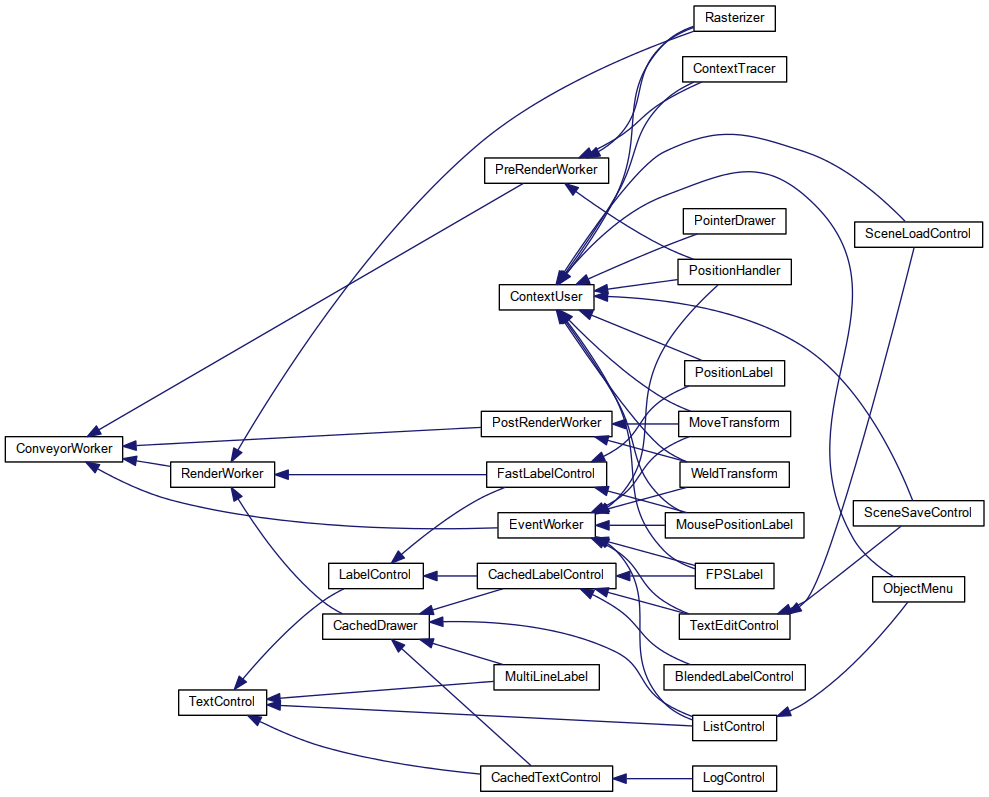
\includegraphics[width=\textwidth]{inherit_graph_73}
\caption{Иерархия обработчиков}
\label{conveyor_hierarchy_dia}
\end{figure}

\subsubsection{Окно}
В программе используется класс окна, который инициализирует графическую библиотеку и содержит основной цикл программы. В нём создаётся окно и устанавливаются начальные элементы управления и блоки настроек. Окно содержит в себе также очередь обработчиков, создаёт контекст и инкапсулирует несколько классов, вроде растеризатора и таймера, ограничивающего время шага. Оно является следующим уровнем в иерархии после точки входа и контроллирует выполнение всей программы.

\subsubsection{Контекст}
Контекст --- структура данных, используемая и модифицируемая на общих основаниях многими обработчиками в конвейере. Контекст содержит в себе всю информацию о сцене, указатели на различные данные, расчитываемые в растеризаторе и используемые другими обработчиками, модели, камеру и прочее. Контекст созадётся классом Window и уничтожается им же, однако указатель на него передаётся всем обработчикам, унаследовавшим специальный базовый класс ContextUser. С помощью него любой обработчик может отредактировать сцену, узнать положение камеры пользователя и многое другое. В частности, в контексте хранится указатель на точки и данные, полученные растеризатором в ходе шага предотрисовки, которые используются затем, например, обработчиком --- трассировщиком для определения объекта, на который в настоящий момент направлен взгляд пользователя. В контексте также есть указатель на окно, через который можно получить и установить многие необходимые величины (высоту и ширину области отрисовки, указатель и его захват и прочее).

\subsubsection{Шаг событий}
Первый шаг конвейера называется шагом событий. Во время этого шага класс Окно принимает события из очереди событий SDL и ретранслирует их всем классам-обработчикам, унаследовавшим базовый класс EventWorker. На некоторые события также предусмотрен отклик со стороны своего окна, например на событие изменение размера окна --- установка нового видеорежима, на запрос выхода из программы --- остановка программы. Каждый класс после обработки события возвращает булевую переменную. Если значение переменной ``истина'', это означает что данное событие обработано полностью и его не следует пускать дальше по конвейеру. Таким образом, более новые обработчики могут перекрывать действие более старых, что даёт возможность, например, некоторым элементам управления перехватывать и обрабатывать движения мыши до основного обработчика. Последним в целочке классов-обработчиков события принимает основной обработчик событий, который реализует основной интерфейс программы. Он отвечает за работу всех горячих клавиш, а так же за перемещение камеры. В нём для выполнения некоторых действий создаются новые обработчики, которые регистрируются в очереди. \\
После того как все события на данный момент были получены и обработаны, для каждого обработчика событий вызывается метод EventStep, в котором происходит обычно генерация отклика на события, например, перемещение камеры.

\subsubsection{Шаг предотрисовки}
Второй шаг конвейера проходит в обратном порядке и начинается с вызова растеризатора, который проводит преобразования точек объектов, освещения, возможно каких-то предварительных отсечений (например, по нормалям) и оставляет на эти данные указатель в контексте. Затем вызываются обработчики для этого шага для всех остальных работников конвейера в обратном порядке. На этом этапе ещё возможно менять некоторые параметры отрисовки, например, материал для объекта. Например, на данном этапе класс трассировщика обнаруживает треугольник на который смотрит пользователь исходя из данных от конвейера и устанавливает для соответствующего треугольника подмену материала через оверлей. Координаты объектов в этом состоянии менять уже нельзя, поэтому некоторым обработчикам, например, обработчикам трансформаций, приходится ждать шага постотрисовки.

\subsubsection{Шаг отрисовки}
На этом этапе, который также проходит в обратном порядке, для каждого работающего на этом шаге обработчика (начиная с растеризатора) вызывается его метод отрисовки, параметром к которому является плоскость для отрисовки. Более поздние элементы отрисовываются поверх более ранних, таким образом, реализуются элементы управления поверх основной сцены. \\
Автором также был реализован специальный класс CachedDrawer (кэширующий обработчик), который сохраняет сгенерированную своим наследником картинку на протяжении нескольких кадров, пока наследник не оповестит его о необходимости перерисовки картинки. Это сильно экономит время для статичных элементов управления, т.е. текстовых полей. не меняющихся слишком часто надписей и.т.д.

\subsubsection{Шаг постотрисовки}
На этом этапе вызываются различные дополнительные методы. Например, обработчики приобразований сцены используют этот этап чтобы изменить параметры объекта исходя из положения камеры.

\subsubsection{Обходчик треугольника} \label{triangle_traverse_struct_section}
В программе с помощью шаблонного метапрограммирования реализован крайне удобный класс абстрактного обходчика треугольников, который включает в себя все необходимые алгоритмы по обходу, и принимает в качестве аргументов шаблона особые классы, которые хранят в себе интерполируемые значения и имеют методы для продвижения по треугольнику на единицу или некое число, а также их специальные подклассы, которые реализуют обход по горизонтали каждой линии и выполнение некой полезной работы в каждой точке. Несмотря на сложность в реализации такого класса, получающийся из шаблона код очень быстр и оптимизирован. Класс обходчика треугольника используется, в частности, очень активно в растеризаторе, где реализовано сразу несколько обходчиков (для отрисовки с разными параметрами), а также в классе трейсера, который использует его для нахождения пересечения взгляда пользователя с треугольником.

\subsubsection{Растеризатор}
Растеризатор --- обработчик, который всегда находится внизу конвейера. Он действует на шагах предотрисовки и отрисовки. Внутри себя он хранит бинарное дерево --- данные, рассчитанные во время предыдущего кадра. Это используется для уменьшения количества вызовов malloc()/free(), благодаря чему достигается ускорение работы. Во время этапа предотрисовки растеризатор преобразовывает точки, нормали, расчитывает векторы для освещения. Если объект который преобразовывается в настоящий момент уже преобразовывался на прошлом шаге мира, растеризатор находит запись для него в дереве кэша и использует сохранившийся там массивы и списки, избегая переаллокации памяти. \\
В реализации растеризатора активно используются макросы и шаблонное метапрограммирование, чтобы уменьшить количество повторяемого кода и при этом минимизировать количество операций, выполняемых при отрисовке. В частности, шаблонно генерируются методы отсечения по плоскостям, а классы обходчиков по треугольнику, о которых рассказано в~\ref{triangle_traverse_struct_section}. Для минимизации повторения кода с сохранением максимальной скорости используется наследование и inline-функции. Построение классов-отрисовщиков из блоков видно из иерархии на рисунке~\ref{rasterizer_hierarchy_img}.

\begin{figure}[!h]
\centering
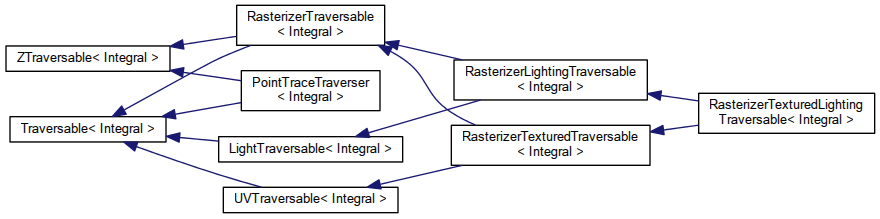
\includegraphics[width=\textwidth]{inherit_graph_117}
\caption{Иерархия отрисовщиков}
\label{rasterizer_hierarchy_img}
\end{figure}

\subsection{Интерфейс программы}
Интерфейс программы выполнен в стиле компьютерной игры с видом от первого лица, который, как считает автор, наиболее подходит для решения данной задачи (рисунок~\ref{main_screenshot}. Сверху окна расположены отладочные данные (лог сообщений и количество кадров в секунду), снизу --- текущая позиция игрока. Все действия в программе выполняются через горячие клавиши, которые по мнению автора крайне удобны для подобного продукта. В программе определено много различных клавиш:
\begin{itemize}
\item W/A/S/D --- передвижение камеры, ``полёт''
\item Numpad 8/4/2/6, указатель мыши --- изменение направления взгляда
\item Space/LCtrl --- изменение высотной составляющей позиции камеры, ``подъём-спуск''
\item G --- включение/отключение захвата мыши программой в положении в центре
\item T --- перемещение и вращение объектов
\item С --- передвижение объекта к другому объекту, ``соединение'' (хотя оба объекта продолжают оставаться самостоятельными)
\item N --- добавление объекта на сцену из списка моделей
\item Y --- удаление объекта со сцены
\item L --- загрузка сцены из файла
\item P --- сохранение сцены в файл
\end{itemize}

\begin{figure}[!h]
\centering
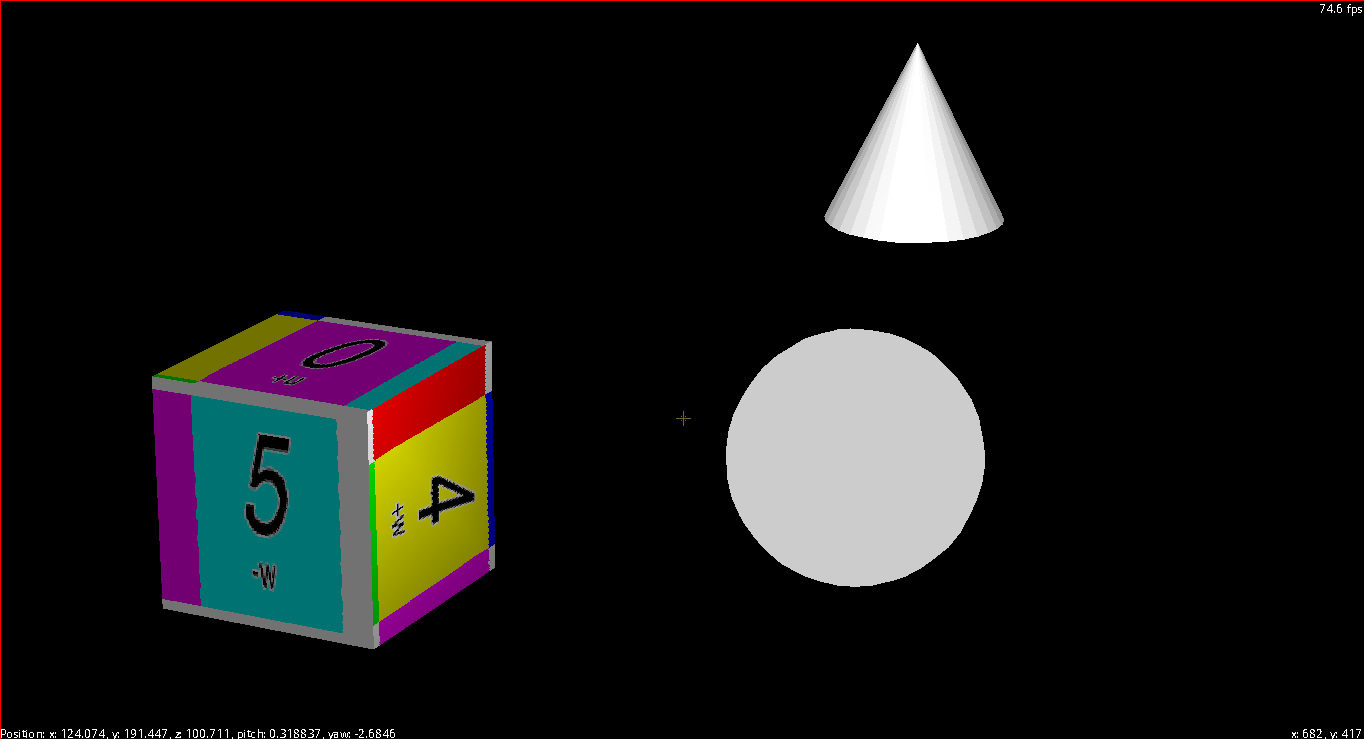
\includegraphics[width=\textwidth]{window}
\caption{Главное окно программы}
\label{main_screenshot}
\end{figure}

\subsubsection{Включение/отключение захвата мыши}
Даёт возможность отключить изменение направление взгляда по движению указателя, и двигать его по видовому экрану свободно, что можно использовать, например, чтобы указать некую сторону объекта, не поворачиваясь.

\subsubsection{Перемещение и вращение объектов}
Объект, на который сейчас направлен взгляд пользователя, становится ``прицепленным'' к камере и двигается в таком положении за камерой пока пользователь не утвердит изменение нажатием левой кнопки мыши или не отменит, нажав Escape. Пользователь может также переключить режим перемещения на вращение, нажав кнопку R (вращение по осям, параллельным плоскости экрана) или Z (вращение по оси, перпендикулярной плоскости экрана). Вращение производится вокруг точки, на которую смотрел пользователь когда начинал операцию.

\subsubsection{``Соединение'' объектов}
Точка, на которую сейчас смотрит пользователь, запоминается. Пользоватею затем предлагается выбрать точку на другом объекте, и эти объекты совмещаются так что эти точки и плоскости на которых они лежат совпадают. Затем пользователь может повернуть прицепляемый объект по оси нормали к плоскости стационарного объекта. Пользователь может утвердить свой выбор нажатием левой кнопки мыши или отклонить нажатием Escape.

\subsubsection{Добавление объектов}
Добавляет в точку, в которой сейчас находится пользователь, новый объект сцены, использующий выбранную пользователем из списка модель. Пользователь может приостановить выбор модели, нажав Escape.

\subsubsection{Удаление объектов}
Объект, на который сейчас направлен взгляд пользователя, удаляется со сцены.

\subsubsection{Загрузка и сохранение сцены}
Пользователю предлагается ввести имя файла, которое затем будет использовано при загрузке или сохранении сцены. При загрузке сцены старая будет безвозвратно утеряна, если ранее не было выполнено сохранение. При возникновении ошибки в области логов появляется соответствующее сообщение.

\newpage
\section{Исследовательский раздел}
В процессе написания программы сохранялась возможность отключения и включения некоторых её оптимизаций и возможностей, на основе чего были проведены некоторые исследования, выражающиеся в замерении скорости работы программы.

\subsection{Оптимизации компилятора}
Компилятор позволяет собирать программу с различными опциями оптимизации --- нас интересуют четыре уровня оптимизации скорости -O0, -O1, -O2 и -O3, а также опция оптимизации \texttt{-ffast-math}, включающая оптимизации работы с числами с плавающей запятой которые могут повлечь потерю точности, \texttt{-funroll-loops}, разворачивающая циклы с постоянным количеством шагов и \texttt{-funswitch-loops}, преобразующий циклы, в которых проверяется не зависящее от цикла условие, в два цикла для разных результатов проверки. \\
Параллельно проводилось сравнение скорости работы программы с использованием собственной библиотеки матриц и векторов по сравнению с библиотекой Eigen3, основным преимуществом которой является использование векторных инструкций процессора, что позволяло одной инструкцией выполнять аналог от нескольких до нескольких десятков обычных инструкций, сгенерированных из собственной библиотеки. \\
Ключи компилятора:
\begin{verbatim}
fstack-protector -funsafe-loop-optimizations -fPIE -mtune=native
  -march=native -fomit-frame-pointer -DGOURAUD_SHADING
  -DAFFINE_TEXTURES -DDUMB_NORMAL_CLIPPING  
\end{verbatim}
Были произведены измерения работы программы на различных уровнях оптимизации с тестовой сценой. Результаты отражены на рисунке~\ref{compiler_optimize_chart}. Результаты показывают влияние уровня оптимизаций на качество конечного кода при активном использовании шаблонного метапрограммирования, особенно хорошо это видно на активно использующей эти возможности внешней библиотеке векторов и матриц. Также этот график демонстрирует прирост производительности при использовании векторных инструкций процессора для работы над матрицами и векторами.

\begin{figure}[!h]
\centering
\begin{tikzpicture}
\begin{axis}[
  ybar,
  bar width=20pt,
  ylabel={FPS},
  enlarge x limits=0.25,
  width=0.75 \textwidth,
  symbolic x coords={-O0, -O1, -O2, -O3},
  xtick=data,
  legend style={at={(0.5,-0.15)},
    anchor=north,legend columns=-1},
  nodes near coords
]

\addlegendentry{Встроенная библиотека};
\addplot
coordinates {(-O0, 27.1) (-O1, 67.1) (-O2, 68.1) (-O3, 70.0)};
\addlegendentry{Eigen3};
\addplot
coordinates {(-O0, 9.2) (-O1, 75.0) (-O2, 79.3) (-O3, 80.1)};
\end{axis}
\end{tikzpicture}
\caption{Сравнение оптимизаций скорости}
\label{compiler_optimize_chart}
\end{figure}

На рисунке также видно, что уровень оптимизации -O0 даёт на выходе крайне неоптимальный код, а уровни -O2 и -O3 практически неотличимы по скорости кода. Это связано с тем, что -O3 добавляет к -O2 лишь несколько небезопасных оптимизаций, которые проявляются хорошо в специфических случаях. \\
В дальнейшем все измерения проводились на уровне оптимизации -O3 с применением внешней библиотеки, что позволяло эффективно разворачивать код, сгенерированный с помощью шаблонов, встраивать небольшие функции прямо в код вызывающей процедуры, и оптимизировало прочие узкие но неинтересные для нас места (в частности операции над векторами и матрицами, которые во внешней библиотеке оптимизированы с применением ассемблерных вставок). Рассмотрим роль дополнительных оптимизаций для выбранной нами конфигурации. Результаты примерения различных оптимизаций приведены на рисунке~\ref{compiler_extra_chart}.

\begin{figure}[!h]
\centering
\begin{tikzpicture}
\begin{axis}[
  ybar,
  ytick=\empty,
  bar width=20pt,
  ylabel={FPS},
  enlarge x limits=0.25,
  legend style={at={(0.5,-0.15)},
    anchor=north,legend columns=-1},
  xtick=data,
  nodes near coords
]

\addlegendentry{Исходные};
\addplot coordinates {(0, 80.1)};
\addlegendentry{-ffast-math};
\addplot coordinates {(0, 80.5)};
\addlegendentry{-funroll-loops};
\addplot coordinates {(0, 80.6)};
\addlegendentry{-funswitch-loops};
\addplot coordinates {(0, 81.3)};
\end{axis}
\end{tikzpicture}
\caption{Дополнительные оптимизации компилятора}
\label{compiler_extra_chart}
\end{figure}

Оптимизация -funroll-loops считается спорной, поскольку программа начинает занимать больше места в памяти (и в кэше процессора), и современные процессоры конвейерно оптимизируют подобные циклы. В итоге в финальные параметры сборки были добавлены \texttt{-ffast-math -funswitch-loops}, что согласно нашему исследованию положительно влияет на скорость программы.

\subsection{Интерполяция текстур}
Было сравнено качество картинки и скорость работы программы при использовании разных способов интерполяции текстур --- афинного и перспективного. Сравнение скорости приведено на графике~\ref{texture_benchmark}. Сравнение картинки можно видеть на \ref{texture_screen}.

\begin{figure}[!h]
\centering
\begin{tikzpicture}
\begin{axis}[
  ybar,
  ytick=\empty,
  bar width=20pt,
  ylabel={FPS},
  enlarge x limits=0.25,
  legend style={at={(0.5,-0.15)},
    anchor=north,legend columns=-1},
  xtick=data,
  nodes near coords
]

\addlegendentry{Без текстуры};
\addplot coordinates {(0, 84.0)};
\addlegendentry{Афинная интерполяция};
\addplot coordinates {(0, 73.5)};
\addlegendentry{Перспективная интерполяция};
\addplot coordinates {(0, 80.6)};
\end{axis}
\end{tikzpicture}
\caption{Скорость интерполяции текстур}
\label{texture_benchmark}
\end{figure}

\begin{figure}[!h]
\centering
\subfloat[][Афинная интерполяция]{
  \centering
  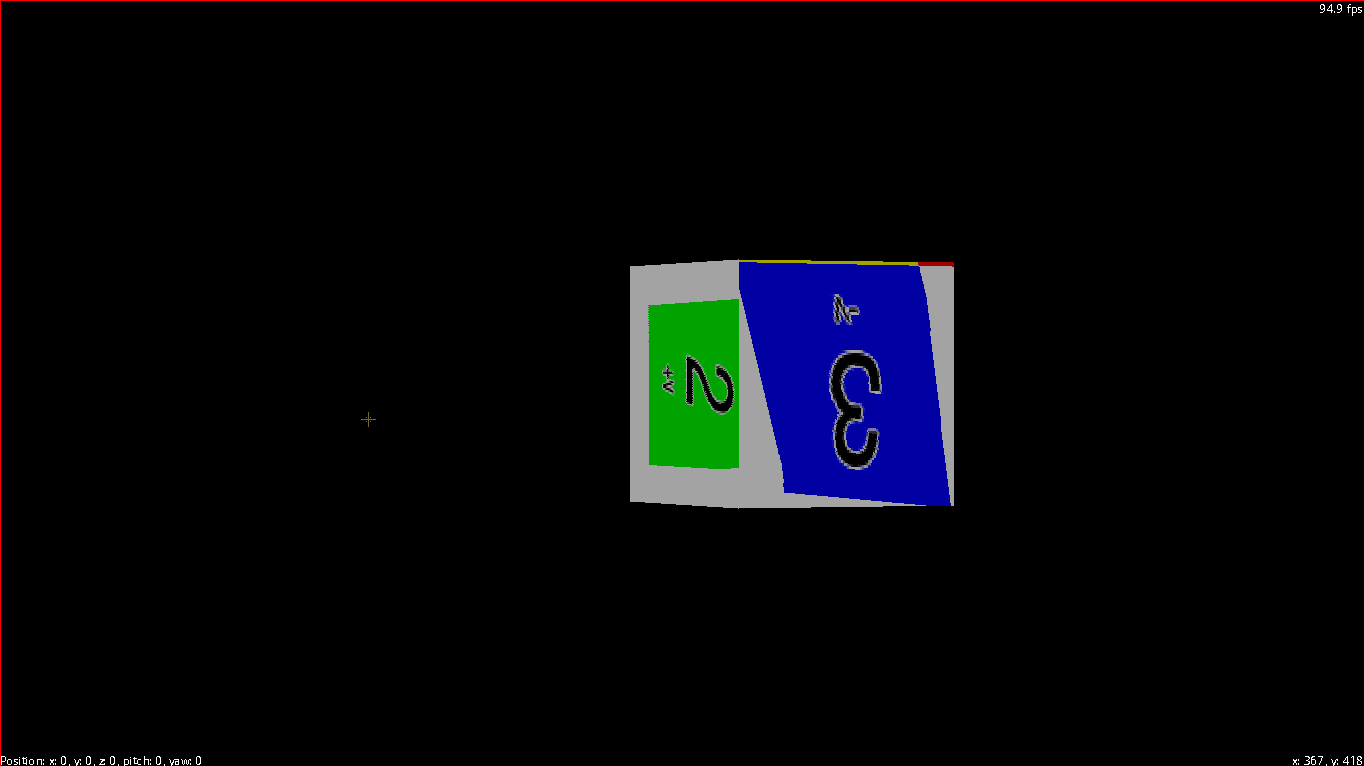
\includegraphics[width=0.45 \textwidth]{texture_affine}
}
\subfloat[][Перспективная интерполяция]{
  \centering
  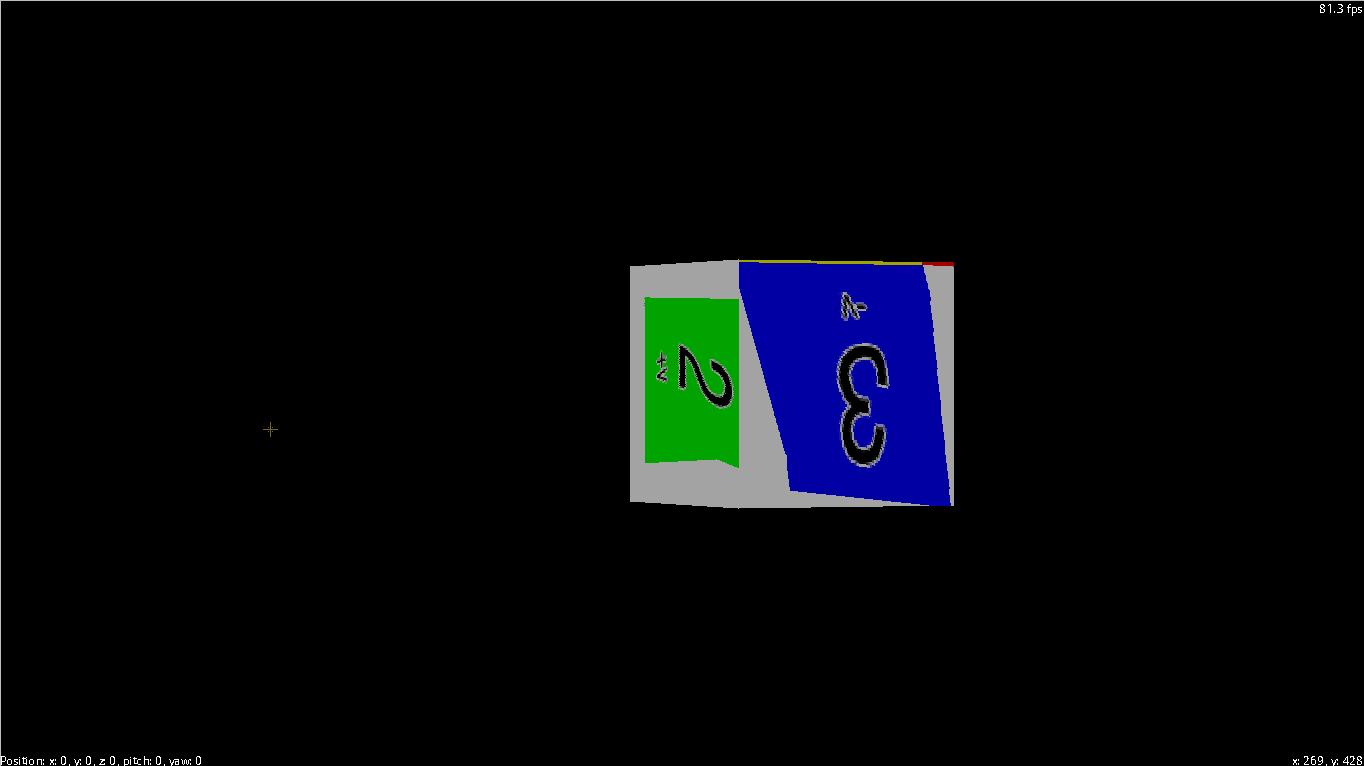
\includegraphics[width=0.45 \textwidth]{texture_perspective}
}
\caption{Сравнение вида текстур}
\label{texture_screen}
\end{figure}

\subsection{Отсечение по нормалям}
Была сравнена скорость работы при использовании трёх видов отсечения по нормалям:
\begin{itemize}
\item Отсутствие отсечения
\item Грубое отсечение (без учёта перспективы)
\item Отсечение с учётом перспективы
\end{itemize}
Сравнение скорости работы программы представлено на рисунке~\ref{normal_clipping_bench}.

\begin{figure}[!h]
\centering
\begin{tikzpicture}
\begin{axis}[
  ybar,
  ytick=\empty,
  bar width=20pt,
  ylabel={FPS},
  enlarge x limits=0.25,
  legend style={at={(0.5,-0.15)},
    anchor=north,legend columns=-1},
  xtick=data,
  nodes near coords
]

\addlegendentry{Без отсечения};
\addplot coordinates {(0, 57.2)};
\addlegendentry{Грубое отсечение};
\addplot coordinates {(0, 73.5)};
\addlegendentry{Отсечение с перспективой};
\addplot coordinates {(0, 70.7)};
\end{axis}
\end{tikzpicture}
\caption{Скорость с отсечением по нормалям}
\label{normal_clipping_bench}
\end{figure}

Из графика видно, насколько существенный прирост скорости даёт отсечение по направлению нормали. Следует учитывать, что при использовании грубого отсечения проявляются достаточно заметные дефекты исчезновения граней тел, которые проецируются на экран ближе к его краям. В итоге, лучше использовать отсечение с учётом перспективы, чтобы не терять в качестве картинки.

\subsection{Тонирование}
В программе сравнивалось качество различных алгоритмов тонирования:
\begin{itemize}
\item Без учёта освещения
\item Плоская тонировка
\item Тонировка по Гуро
\item Тонировка по Фонгу
\end{itemize}
Сравнивалось как качество картинки, так и скорость работы программы при выбранной тонировке. Результаты по скорости работы представлены на графике~\ref{shading_benchmark}, а сравнение по качеству --- на рисунке~\ref{shading_comparison}.

\begin{figure}[!h]
\centering
\begin{tikzpicture}
\begin{axis}[
  ybar,
  ytick=\empty,
  bar width=20pt,
  ylabel={FPS},
  enlarge x limits=0.25,
  legend style={at={(0.5,-0.15)},
    anchor=north,legend columns=-1},
  xtick=data,
  nodes near coords
]

\addlegendentry{Без тонировки};
\addplot coordinates {(0, 100.8)};
\addlegendentry{Плоское освещение};
\addplot coordinates {(0, 80.3)};
\addlegendentry{Тонировка по Гуро};
\addplot coordinates {(0, 73.5)};
\addlegendentry{Тонировка по Фонгу};
\addplot coordinates {(0, 39.0)};
\end{axis}
\end{tikzpicture}
\caption{Скорость тонировки}
\label{shading_benchmark}
\end{figure}

\begin{figure}[!h]
\centering
\subfloat[][Без тонировки]{
  \centering
  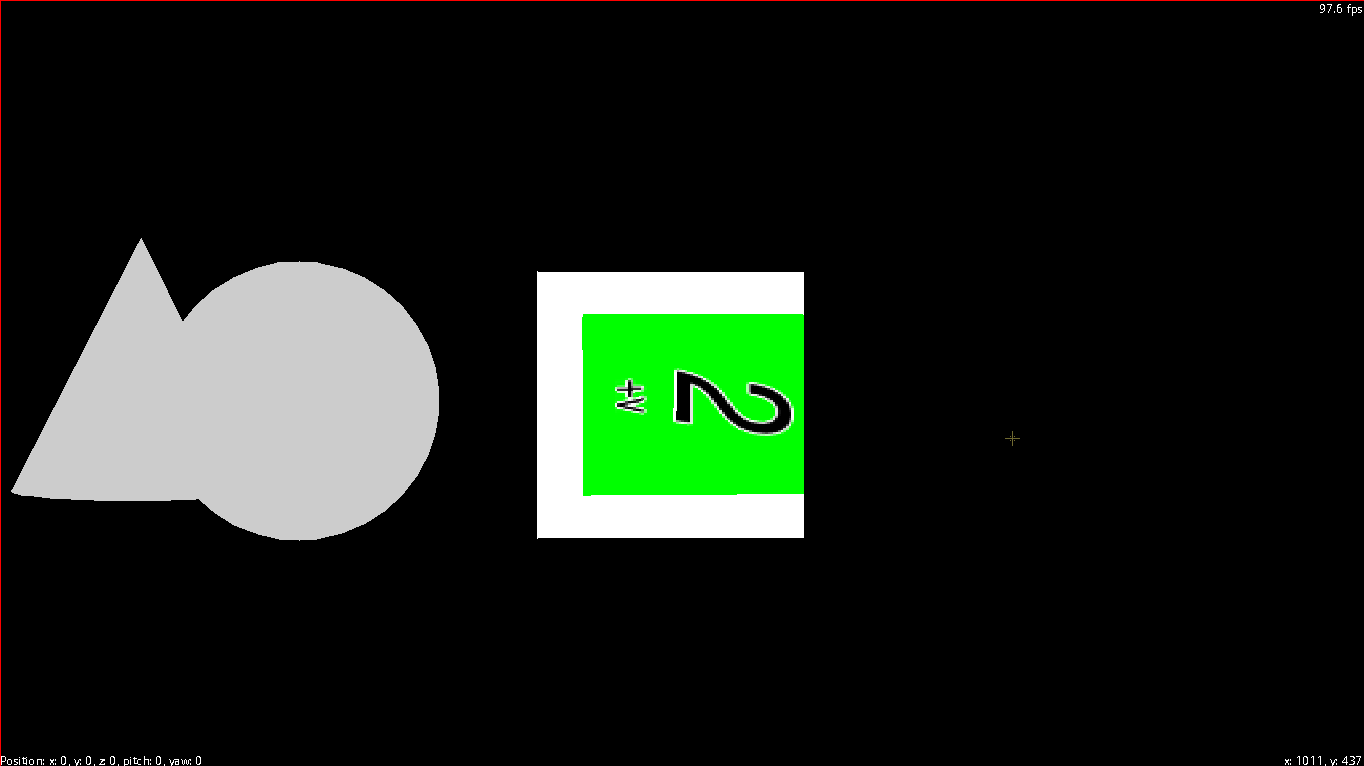
\includegraphics[width=0.45 \textwidth]{no_shading}
}
\qquad
\subfloat[][Плоское освещение]{
  \centering
  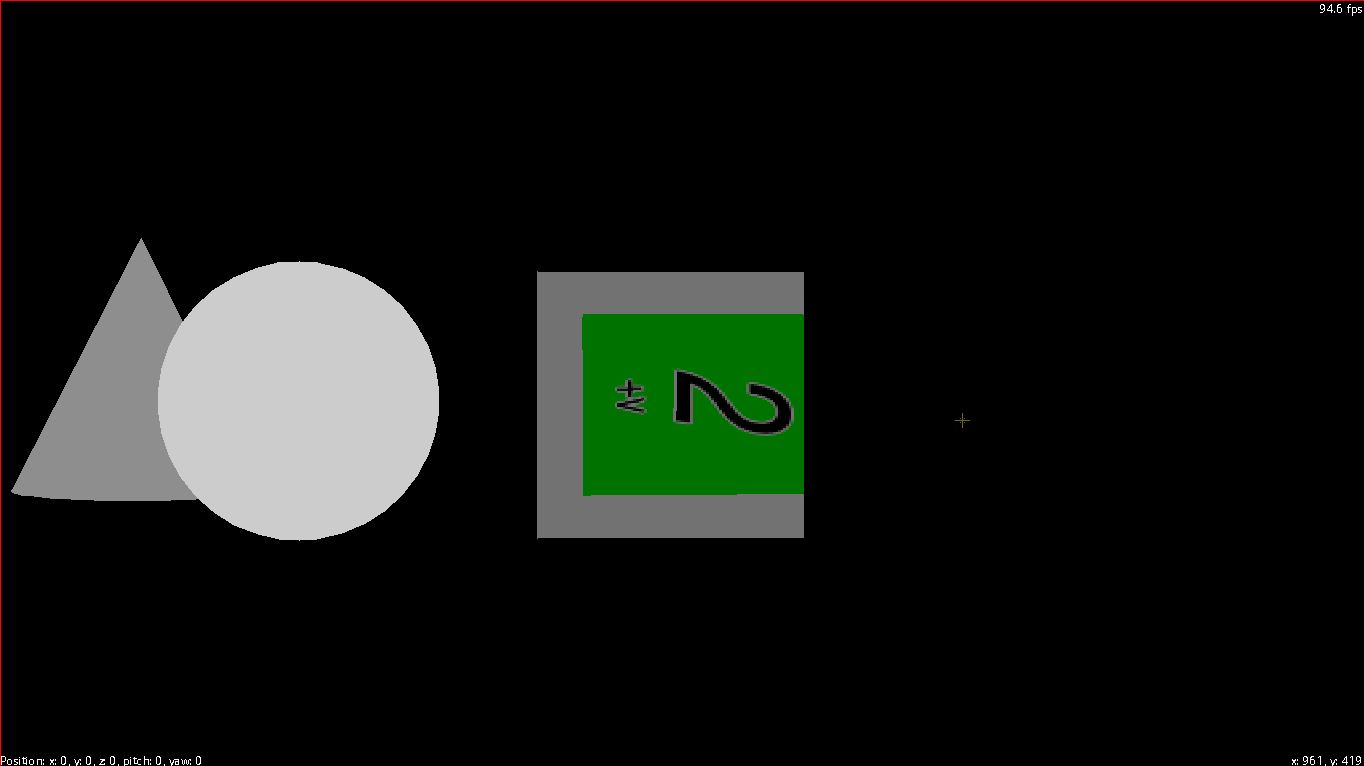
\includegraphics[width=0.45 \textwidth]{flat_shading}
}
\subfloat[][Тонировка по Гуро]{
  \centering
  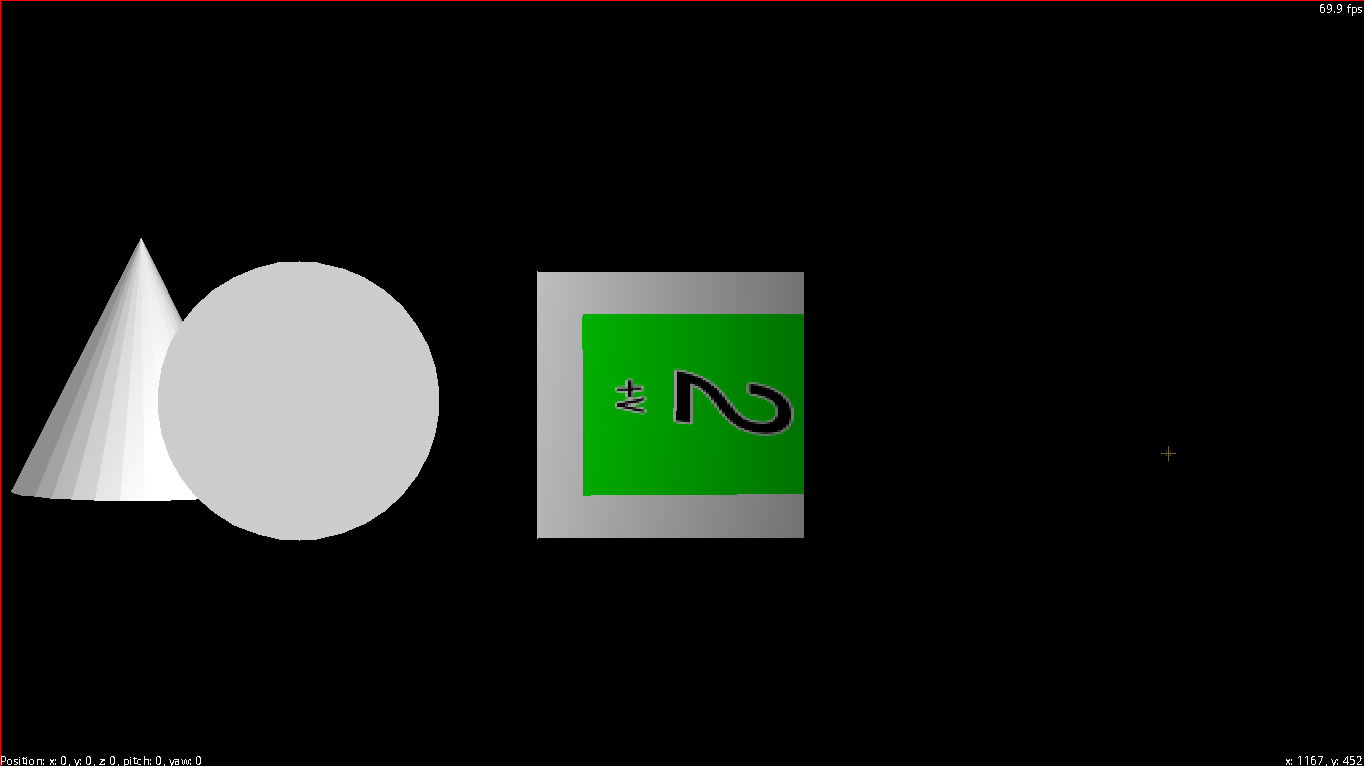
\includegraphics[width=0.45 \textwidth]{gouraud_shading}
}
\qquad
\subfloat[][Тонировка по Фонгу]{
  \centering
  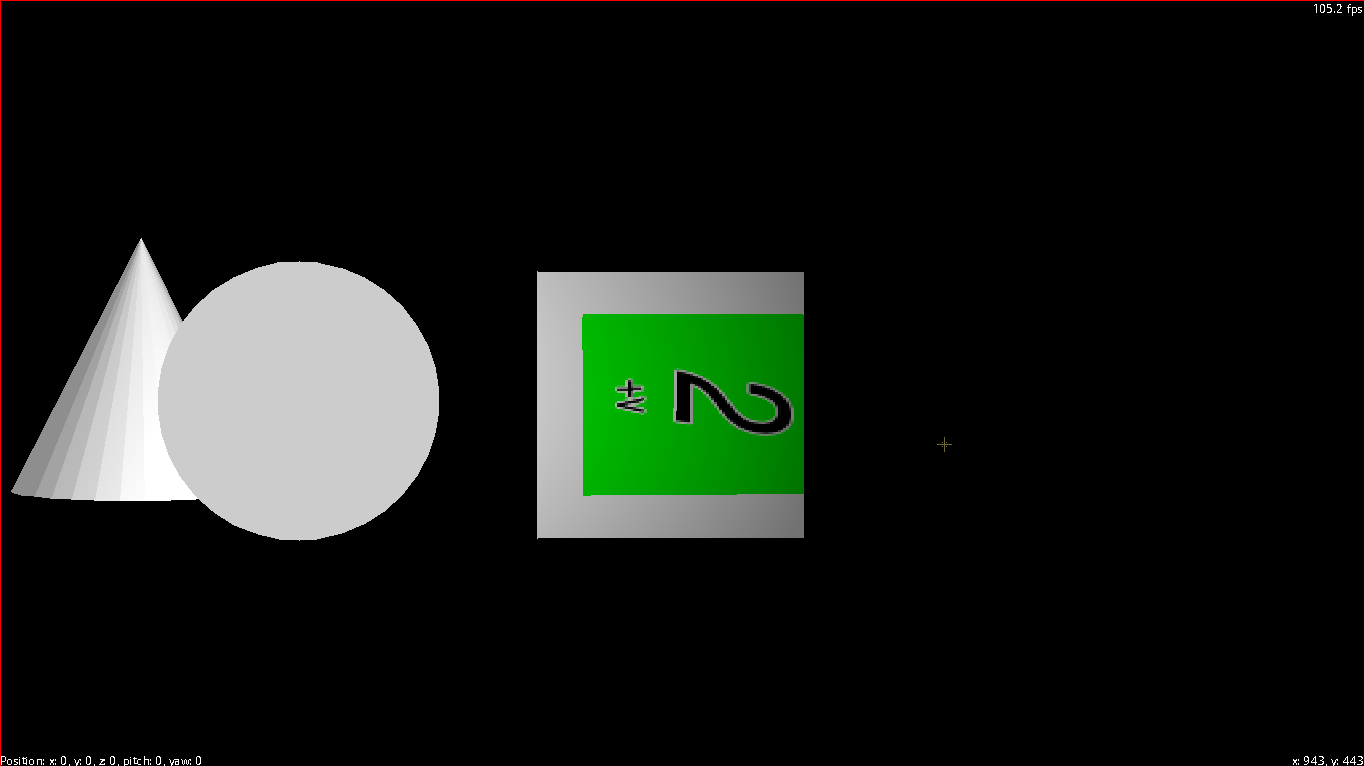
\includegraphics[width=0.45 \textwidth]{phong_shading}
}
\caption{Сравнение вида текстур}
\label{shading_comparison}
\end{figure}

Для высокополигональной модели тонировка по Фонгу и по Гуро не будут так уж сильно различаться, хотя тонировка по Фонгу медленнее почти в два раза. Плоская тонировка не даёт большого прироста качества по сравнению с отсутствием тонировки, но при этом даёт большое падение производительности. В итоге, оптимальными для приложения реального времени оказались два режима --- отсутствие освещения как такового и тонировка по Гуро, дающая хорошее качество тонировки.

\section*{Заключение}
В ходе разработки проекта был изучен набор алгоритмов машинной графики для отрисовки трёхмерных объектов в реальном времени, изучены новые возможности языка C++ и его подмножества C++11, изучено и применено несколько сторонних библиотек, создано несколько полезных библиотек для будущих проектов, отточены навыки программирования и использования некоторых технических средств. Итогом работы является целиком завершённая программа, а также некоторый исследовательский материал на её основе. В целом, работа выполнена успешно.

\newpage
\printbibliography[heading=bibintoc]

\end{document}
